\documentclass[a5paper,10pt,pagesize,DIV=classic]{scrbook}
\usepackage[pass]{geometry}

\usepackage{graphicx}

\usepackage[utf8]{inputenc} 
\usepackage[russian]{babel}

\usepackage{amsthm}
\usepackage{hyperref}

\begin{document}

\title{Учебник по математике}
\author{Роман Добровенский\\ \\heller@heller.ru\\http://heller.ru}
\date{2012, Москва}
\maketitle

\tableofcontents

\chapter*{Введение}
\addcontentsline{toc}{chapter}{Введение}

Эта книга изначально замышлялась как простой учебник для новичков в математике. После первых двух глав (которые планировалось сделать коротким введением и обзором, но в итоге они разрослись на сотню страниц) стало понятно, что этот учебник понимают только единицы. Увы. Тем не менее, учебник я продолжаю писать и буду по мере возможностей его перерабатывать, чтобы сделать более доступным.

Пока можно порекомендовать обращаться к отдельным главам учебника и читать материал поверхностно. Если что-то понятно~--- замечательно. Если непонятно~--- не беда. Либо это вам и не нужно, либо прочитаете то же самое в другом месте на более простом, менее научном языке. Несмотря на сложность, я считаю, что в принципе чтение его может оказаться полезным, в том числе и самым новичкам.

Учебник пишется на чистом энтузиазме, распространяется свободно и без ограничений.

Для скачивания всегда доступна последняя версия pdf-файла здесь: \url{http://heller.ru/tutorial.pdf}

Исходные коды в \LaTeX{} могут быть скачаны на GitHub: \linebreak
\url{http://github.com/xHellerx/Math-tutorial}

Учебнику всегда требуется помощь с поиском ошибок в тексте (опыт показывает, что их полно) и с общей критикой. Также требуется помощь с вёрсткой. Если вы хорошо разбираетесь в \LaTeX, я был бы признателен за помощь с оформлением, так как у меня у самого с этим очень плохо. В-третьих, было бы полезно распространение информации о курсе. Посоветуйте его в своём блоге, своим студентам, родителям и соседям.


\chapter{Логика}
Первая глава дает несколько неформальное описание основных законов логики. Главная цель этой главы дать какую-то интуицию об излагаемых понятиях и о принципах логических выводов, прежде чем мы все это формализуем и используем в конце второй главы. Если вам не особо интересны основания математики, то вы можете сразу переходить к середине третьей главы и читать более прикладные вещи, обращаясь сюда по необходимости как к справочнику.

Наиболее важными являются первый и четвертый параграфы. Остальные вези уже имеют более факультативный характер. Если у вас будут проблемы с пониманием первых параграфов, попробуйте сразу решать упражнения в конце.

\section{Базовые понятия}

\term{Высказыванием} мы будем называть любую осмысленную фразу русского языка. Например: «На улице идёт дождь», «Девки гуляют по улице», <<Вася тонировал свою \glqqшестёрку\grqq>>. В рамках науки математической логики мы правда ограничимся лишь теми высказываниями, про которые можно однозначно судить, \term{истинны} они или \term{ложны} (мы можем этого не знать, но важно, что сама постановка фразы допускает однозначную трактовку высказывания).

Истинные высказывания мы будем обозначать символом $1$, а ложные~--- символом $0$. В общем-то, нас даже не будет интересовать сам физический смысл высказывания, лишь его истинность~--- справедливость всех логических законов и операций, о~которых мы будем говорить, не зависит от содержания самих высказываний и оперирует лишь с понятием истинности.

Сами высказывания мы будем обозначать какими-нибудь буквами какого-нибудь алфавита (использовать ли заглавные или строчные, английские или греческие символы, совершенно не принципиально~--- в разных частях курса мы будем использовать разные соглашения, исходя из соображений удобства). Например, запись $a = 1$ обозначает, что $a$~--- это некоторое истинное высказывание. Повторюсь, что смысл высказывания нас не интересует, оно может быть по сути любым, лишь бы было истиной.

Определим теперь простейшие логические операции (они же называются логическими связками). Пусть для начала высказывание $a$ имеет конкретный смысл «на улице идёт дождь», а высказывание $b$ имеет смысл «на улице много машин». К этим двум высказываниям можно применить логическую связку (операцию) «И», и в итоге мы получим высказывание «на улице идёт дождь и много машин».

На языке математики логическая связка «И» обозначается символом $\land$, а результат применения этой связки к нашим двум высказываниям записывается как $a\land b$. (Вообще научно «И» \mbox{также} называется \term{конъюнкцией}, но это знать и помнить совершенно не обязательно.) Давайте теперь рассмотрим истинность этого высказывания. Если это правда, что на улице много машин, и также правда, что на улице идет дождь, то и наше высказывание «на улице много машин и идёт дождь» будет правдой. Если же хотя бы одно из этих утверждений ложно, то и наша фраза $a \land b$ будет ложной: если на улице нет дождя, то не является правдой и составное высказывание «на улице идёт дождь и много машин».

Определение логической связки «И» можно резюмировать следующей таблицей:

\begin{table}[h]
\centering
\begin{tabular}{c c | c}
$a$ & $b$ & $a \land b$ \\
\hline
0 & 0 & 0 \\
0 & 1 & 0 \\
1 & 0 & 0 \\
1 & 1 & 1
\end{tabular}
\caption{Определение логической связки <<И>>}\label{table:logic-and}
\end{table}


Подобные таблицы называются таблицами истинности. В них перечислены все возможные логические значения интересующих нас высказываний и результат применения к ним логической связки. Что-то типа таблицы умножения.

В полной аналогии с операцией «И» можно определить следующие базовые операции:

\begin{itemize}
\item Операция «ИЛИ», она же «И/ИЛИ», она же \term{дизъюнкция} (запоминать это слово не нужно), обозначается как $\lor$. Выражение $a\lor b$ истинно, когда истинно хотя бы одно из высказываний $a$ или $b$.
\item Операция «Исключающее ИЛИ», по-английски называется «eXclusive OR», или кратко «XOR». По-русски её для краткости часто называют «ксор» или --- в глагольной форме --- «ксорить», хотя слово это, конечно, сленговое и совершенно непечатное. Обозначается данная операция как $\oplus$. Высказывание $a \oplus b$ истинно только тогда, когда истинно лишь одно из высказываний $a$ или $b$, но не оба сразу.
\item Операция «Эквиваленция». Обозначается как $a \leftrightarrow b$. Высказывание $a \leftrightarrow b$ истинно, когда $a$ и $b$ либо одновременно истинны, либо одновременно ложны.
\item Операция «НЕ», она же «Отрицание». Обозначается как $\neg$. Высказывание $\neg a$ истинно тогда, когда $a$ ложно, и наоборот.
\item Операция <<Импликация>>, она же <<Следствие>>. Обозначается как $a \to b$. Высказывание $a \to b$ истинно либо когда одновременно и $a$, и $b$ истинны, либо когда $a$ ложно.
\end{itemize}

Всё сказанное, возможно, станет более понятно, когда мы выразим все операции одной таблицей истинности:

\begin{table}[h]
\centering
\begin{tabular}{cc|cccccc}
$a$ & $b$ & $a\land b$ & $a\lor b$ & $a\oplus b$ & $a\leftrightarrow b$ & $\neg a$ & $a \to b$\\
\hline
0 & 0 & 0 & 0 & 0 & 1 & 1 & 1 \\
0 & 1 & 0 & 1 & 1 & 0 & 1 & 1 \\
1 & 0 & 0 & 1 & 1 & 0 & 0 & 0 \\
1 & 1 & 1 & 1 & 0 & 1 & 0 & 1
\end{tabular}
\caption{Сводная таблица истинности логических операций}
\end{table}

Обратите внимание на то, что в естественном языке фраза «на улице идёт дождь или много машин» не особо хорошо определена~--- непонятно, имеется ли в виду «или то, или другое» (исключающее <<ИЛИ>>), или же «и то, и другое». В математике эти два смысла строго разграничены операциями $\lor$ и $\oplus$.

Также стоит уточнить смысл операции эквиваленции~--- она в~действительности ничего не говорит о реальной связи между высказываниями, лишь об их истинности. Так, любые два заведомо ложных высказывания оказываются эквивалентны: «Компьютеры не умеют умножать числа» $\leftrightarrow$ «Солнце вращается вок\-руг Земли». То же и с заведомо истинными высказываниями: «Компьютеры считают лучше людей» $\leftrightarrow$ «Земля вращается вок\-руг Cолнца». Это может несколько сбивать с толку поначалу, но более ясен смысл эквиваленции станет несколько позже, когда мы будем говорить о моделях.

Определение импликации может показаться довольно непонятным, по крайней мере сразу не ясно, почему именно при ложном $a$ должно быть истинно любое следствие $a\to b$. Такое определение действительно не слишком логично, и причины такого определения связаны скорее не с самой логикой, а с формальной необходимостью. Откуда растут корни именно такого \mbox{определения,} мы рассматрим в следующем параграфе, а также в двух параграфах о теориях, а пока же примем определение импликации просто как есть и будем относиться к ней как к~арифметической операции без какой-либо специальной мотивации.

Используя перечисленные операции, можно задавать и довольно сложные высказывания, например, что-то вроде такого:
$$
((a \lor b) \leftrightarrow (c \land a)) \oplus b.
$$

Круглыми скобками мы обозначаем порядок, в котором выполняются операции. Если для каждого из высказываний $a$, $b$ и~$c$ определить, истинно оно или ложно, то по таблице истинности можно определить, истинно ли всё высказывание.

Пусть, например, $a$ истинно, а $b$ и $c$ ложны. Тогда, подставив вместо этих высказываний $1$ и $0$ в приведённую формулу и воспользовавшись правилами из таблицы истинности, можно установить истинность и всего высказывания:
$$
((1 \lor 0) \leftrightarrow (0 \land 1)) \oplus 0 = (1 \leftrightarrow 0) \oplus 0 = 0 \oplus 0 = 0.
$$

В итоге наше высказывание оказалось ложно при данных значениях истинности для $a$, $b$ и $c$. Если же, например, все три высказывания будут ложными, то всё высказывание окажется истинным:
$$
((0 \lor 0) \leftrightarrow (0 \land 0)) \oplus 0 = (0 \leftrightarrow 0) \oplus 0 = 1 \oplus 0 = 1.
$$

Приведённые примеры уже больше напоминают какую-то скорее безумную арифметику с двумя цифрами, нежели логику, и наделить каким-то бытовым смыслом приведённые формулы, кажется, уже сложно, но подобные примеры необходимы для того, чтобы понять, как вообще со всеми этими понятиями работать. Позже мы будем рассматривать более осмысленные примеры, пока же мы слишком мало знаем и привести что-то осмысленное сложно.

Однако пора доказать нашу первую теорему.

\begin{thm} Для логических операций справедливы следующие законы:

\subparagraph{Ассоциативность:}
\begin{enumerate}
\item $(a \land b) \land c = a \land (b \land c)$,
\item $(a \lor b) \lor c = a \lor (b \lor c)$,
\item $(a \oplus b) \oplus c = a \oplus (b \oplus c)$.
\end{enumerate}

\subparagraph{Коммутативность:}
\begin{enumerate}
\item $a \land b = b \land a$,
\item $a \lor b = b \lor a$,
\item $a \oplus b = b \oplus a$,
\item $a \leftrightarrow b = b \leftrightarrow a$.
\end{enumerate}

\subparagraph{Дистрибутивность:}
\begin{enumerate}
\item $a \land (b \lor c) = (a \land b) \lor (a \land c)$,
\item $a \lor (b \land c) = (a \lor b) \land (a \lor c)$,
\item $a \land (b \oplus c) = (a \land b) \oplus (a \land c)$.
\end{enumerate}

\subparagraph{Двойное отрицание:}
\begin{enumerate}
\item $\neg\neg a = a$.
\end{enumerate}

\subparagraph{Закон исключенного третьего:}
\begin{enumerate}
\item $a \lor \neg a = 1$,
\end{enumerate}

\subparagraph{Закон противоречия:}
\begin{enumerate}
\item $a \land \neg a = 0$,
\end{enumerate}

\subparagraph{Законы де Моргана:}
\begin{enumerate}
\item $\neg (a \land b) = (\neg a) \lor (\neg b)$,
\item $\neg (a \lor b) = (\neg a) \land (\neg b)$.
\end{enumerate}

\subparagraph{Ещё по мелочам:}
\begin{enumerate}
\item $a \land 1 = a$,
\item $a \land 0 = 0$,
\item $a \lor 1 = 1$,
\item $a \lor 0 = a$,
\item $a \oplus 0 = a$,
\item $a \oplus 1 = \neg a$,
\item $\neg (a \oplus b) = (a \leftrightarrow b)$,
\item $a \oplus \neg a = 1$,
\item $a\land a = a$,
\item $a \lor a = a$,
\item $a \oplus a = a$,
\item $a \land (\neg a \lor b) = a \land b$,
\item $a \lor (\neg a \land b) = a \lor b$.
\end{enumerate}

\subparagraph{Для импликации:}
\begin{enumerate}
\item $a \rightarrow b = b \vee \neg a$
\item $\neg(a \rightarrow b) = a \wedge \neg b$
\item $a \rightarrow a$
\item $a \leftrightarrow b = (a \rightarrow b) \wedge (b\rightarrow a)$
\item Транзитивность: $((a \rightarrow b) \wedge (b \rightarrow c)) \rightarrow (a \rightarrow c)$
\item $(a \vee b) \wedge (\neg a \vee c) \rightarrow b \vee c$
\item $(a \rightarrow b \wedge c) \rightarrow (a \rightarrow b)$
\item $a \rightarrow b = \neg b \rightarrow \neg a$
\end{enumerate}
\end{thm}

\begin{proof}
Каждую из формул я доказывать не буду, поскольку все они доказываются аналогично и я настоятельно рекомендую провести доказательство самостоятельно. Я лишь продемонстрирую на отдельных примерах, как это делается.

Подходов тут существует три:
\begin{itemize}
\item Интуитивный. Ассоциативность и коммутативность операций «И» и «ИЛИ» на самом деле очевидна. Вообще, конечно, говорить «очевидно» в математике мы не имеем права, поскольку очевидное часто оказывается неверным и наоборот. Однако в подобных совсем уж тривиальных случаях строго доказывать каждую теорему будет утомительно. Если утверждение теоремы у вас не вызывает сомнения, и вы знаете, как его можно строго проверить~--- можно и не париться.
\item Выводить одно из другого, применяя к начальной формуле другие сформулированные нами формулы. Например, вот как можно вывести последнюю формулу в нашем списке, воспользовавшись дистрибутивностью:
$$
a \lor (\neg a \land b) = (a \lor \neg a) \land (a \lor b) = 1 \land (a \lor b) = a \lor b.
$$

\item Самый тупой и простой способ~--- просто перебрать все возможные варианты, построив таблицу истинности. В таблице 1.3 демонстрируется, как таким образом возможно доказать закон дистрибутивности. Собственно, что и требовалось доказать (следующий за этим предложением значок будет всегда в дальнейшем означать конец доказательства).

\begin{table}[h]
\centering
\begin{tabular}{ccc|cc|ccc}
$a$&$b$&$c$&$b\lor c$&$a\land(b\lor c)$&$a\land b$&$a\land c$&$(a\land b)\lor(a\land c)$\\
\hline
0&0&0&0&0&0&0&0\\
0&0&1&1&0&0&0&0\\
0&1&0&1&0&0&0&0\\
0&1&1&1&0&0&0&0\\
1&0&0&0&0&0&0&0\\
1&0&1&1&1&0&1&1\\
1&1&0&1&1&1&0&1\\
1&1&1&1&1&1&1&1
\end{tabular}
\caption{Доказательство дистрибутивности логических операций}
\end{table}

\end{itemize}
\end{proof}

К сожалению, то, что перебор нам тут помог доказать что-то~--- редкое исключение. Кроме как для почти тривиальных логических соотношений метод перебора в математике не годится, поскольку обычно перебирать придётся слишком много значений, с чем никакой компьютер не справится. И это в лучшем случае~--- часто значений, которые придётся перебрать, будет вооб\-ще беско\-неч\-но много, или даже ещё больше.

Из приведённой теоремы важно выделить законы ассоциативности и дистрибутивности. Закон ассоциативности по сути утверждает, что для перечисленных операций не важно, в каком порядке расставлять скобки и, соответственно, применять операции (чуть более строго мы это обсудим в третьей главе). По этой причине круглые скобки для ассоциативных операций можно вооб\-ще опускать, и следующие выражения оказываются совершенно равнозначны:
$$
(a \lor (b \lor c)) \lor d = (a \lor b) \lor (c \lor d) = a \lor b \lor c \lor d
$$

Закон коммутативности же означает, что нам не важен порядок участвующих в выражении высказываний. В совокупности с ассоциативностью это говорит также, что мало того, что мы можем опускать скобки, мы ещё и порядок можем путать:
$$
(a \lor (b \lor c)) \lor d = b \lor d \lor c \lor a.
$$

На фоне этого может оказаться странным поведение эквиваленции. Как легко убедиться, если построить таблицу истинности, операция эквивалентности тоже является ассоциативной:
$$
(a \leftrightarrow b) \leftrightarrow c = a \leftrightarrow (b \leftrightarrow c).
$$

Тем не менее, если мы будем применять её в таком виде, опустив круглые скобки, то результат может оказаться неожиданным:
$$
(1 \leftrightarrow 0 \leftrightarrow 0) = ((1 \leftrightarrow 0) \leftrightarrow 0) = (0 \leftrightarrow 0) = 1.
$$

Это несколько противоречит интуитивному представлению о понятии «эквивалентность». Нам хотелось бы иметь возможность писать $a \leftrightarrow b \leftrightarrow c$ и ожидать, что данное высказывание будет истинным лишь в том случае, когда все три высказывания либо одновременно истинны, либо одновременно ложны. Это было бы логично.

В математике так и поступают. Если в последовательных операциях эквивалентности не указываются скобки, то имеется в виду следующее:
$$
a \leftrightarrow b \leftrightarrow c = (a \leftrightarrow b) \land (b \leftrightarrow c).
$$

Именно по этой причине закон ассоциативности для эквивалентности обычно не рассматривается. Такая странность возникает из-за некоторой неточности привычного человеческого языка, когда мы, произнося одни и те же слова, можем иногда подразумевать довольно разные логические операции. Это во многом сродни неточности слова «или»: из-за этого нам пришлось разграничивать операции $\lor$ и $\oplus$. Здесь нет никакого парадокса или противоречия~--- это просто надо иметь в виду.

Также замечания заслуживает закон де Моргана. Он на самом деле обобщается на любое количество высказываний. Для примера продемонстрируем простейшую ситуацию:
$$
\neg(a \lor b \lor c) = \neg(a \lor (b \lor c)) = \neg a \land \neg (b \lor c) = \neg a \land \neg b \land \neg c.
$$

Аналогично можно распространить этот закон на любое количество высказываний (даже бесконечное). Как это сделать строго математически, мы обсудим в дальнейшем в нашем курсе, пока же можно просто попробовать развить какую-то интуицию относительно этого закона.

Пусть высказывание $a$ означает, что Тане нравятся бритые мальчики, а высказывание $b$ означает, что Тане нравятся мальчики в спортивных штанах. Предположим, однако, что Таня не дура какая-нибудь, и для неё верно высказывание:
$$
\neg(a \land b) = \text{«Тане не нравятся бритые мальчики в спортштанах»}
$$

(На всякий случай сообщу, что автор текста сам бреется налысо и имеет в гардеробе зауженные спортштаны.)

Приведённое высказывание, однако, не подразумевает, что Тане не подойдёт бритый мужчина в костюме, или же патлатый спортсмен~--- данное высказывание говорит лишь о том, что для нее неприемлемо сочетание «лысый + спортштаны». Довольно косноязычно, но можно всё же утверждать следующее:

\begin{quote}
«Таню устроил бы парень, который хотя бы не лысый или хотя бы не носит спортштаны».
\end{quote}

Если вдуматься, то это ровно та же самая фраза, которую мы назвали первоначально, но она просто перефразирована. И она дословно выражается как $\neg a \lor \neg b$, а это как раз то, что мы ожидали получить по закону де Моргана. Если добавить к первоначальным двум высказываниям ещё какие-то высказывания, характеризующие предпочтения Тани, то мы получили бы тот же закон де Моргана, но уже для многих высказываний.

Подобные интуитивные соображения можно придумать для любой формулы нашей первой теоремы, и хорошо бы это проде\-лать~--- это полезно. С тем же законом де Моргана я впервые столкнулся лет 10 назад (правда не в мат. логике, а в теории вероятностей, которую я пытался читать без какой-либо начальной подготовки), и в книжке, которую я читал, всё, что о нём было сказано, что это «очевидно». Сейчас уже стыдно признаваться, но над этим «очевидным» утверждением мне тогда пришлось поломать голову, прежде чем я смог согласиться с автором в том, что это действительно так.

Из всего списка приведённых в теореме 1.1 утверждений интересно выделить те, что касаются импликации. При том, что таблица истинности для импликации может показаться довольно странной,  она обладает весьма логичными свойствами, которые характерны для интуитивного понятия <<следствия>>. Например, закон транзитивности является отражением простого логического закона: если из $a$ следует $b$, а из $b$ следует $c$, то из $a$ следует $c$. Аналогично равенство $a \rightarrow b = \neg b \rightarrow \neg a$ означает, что если из $a$ следует $b$, и нам известно, что $b$ ложно, то отсюда следует ложность $a$. Таким образом, введённое определение импликации действительно в каком-то смысле отражает операцию <<следствие>>, как мы её понимаем на интуитивном уровне. Эти идеи мы будем развивать в следующих параграфах.

Читателю же я рекомендую доказать каждую из формул приведённой теоремы и продумать больше не над самим фактом справедливости формулы, а над интуитивной интерпретацией.



\section{Представление функций}

В прошлом параграфе мы определили с помощью таблиц истинности пять логических операций. Нам никто не мешает определить и другие операции, задав их таблицу истинности, причём им не обязательно иметь один или два параметра — можно и больше, никто не запрещает. Для примера рассмотрим операцию (удобней, наверное, называть её функцией) $f$ с тремя параметрами, описанную в таблице 1.4. Записывать эту операцию мы будем как $f(a, b, c)$. По таблице легко находить её значения при конкретных параметрах, например: $f(0,0,1) = 0$ или $f(1,0,1) = 1$.

\begin{table}[h]
\centering
\begin{tabular}{ccc|c}
$a$&$b$&$c$&$f$\\
\hline
0&0&0&1\\
0&0&1&0\\
0&1&0&1\\
0&1&1&0\\
1&0&0&1\\
1&0&1&1\\
1&1&0&0\\
1&1&1&0
\end{tabular}
\caption{Представление булевой функции с тремя параметрами}
\end{table}

Какой физический смысл данной функции/операции? Пока никакого — мы делаем то, что мы делаем, просто потому, что мы можем это делать. В математике часто так поступают, а применение это всё находит позже.

Теперь давайте поймём, как определить эту же самую функцию, выразив её через уже известные нам логические операции.

Для начала рассмотрим более простую функцию $g_0$, которая имеет значение $1$ только при наборе параметров $g_0(1, 0, 1)$, а во всех остальных случаях её значением будет $0$. Легко догадаться, что такая функция в точности представляется как: $$g_0(a, b, c) = a\land \neg b \land c.$$ Рассмотрим также функцию $g_1(a, b, c)$, которая принимает значение $1$ только на наборе аргументов $g_1(0, 0, 0)$. Её, соответственно, можно представить как: $$g_1(a, b, c) = \neg a \land \neg b \land \neg c.$$

Теперь рассмотрим функцию $h$, которая принимает значение~$1$ на обоих наборах параметров $(1, 0, 1)$ и $(0, 0, 0)$. Это можно сформулировать так:   значение функции $h$ истинно, когда истинно значение хотя бы одной из функций $g_0$ и $g_1$. Сказанное дословно переносится на язык математической логики следующим образом: $$h(a, b, c) = g_0(a, b, c) \lor g_1(a, b, c).$$

Подставив сюда выражения для $g_0$ и $g_1$, получаем: $$h(a, b, c) = (a\land \neg b \land c) \lor (\neg a \land \neg b \land \neg c).$$

Продолжая рассуждать таким же образом, можно прийти и к выражению для функции $f$, заданной выше таблицей истинности: $$f(a, b, c) = (\neg a \land \neg b \land \neg c) \lor (\neg a \land b \land \neg c)\lor (a \land \neg b \land \neg c) \lor (a\land \neg b \land c). $$

Легко видеть, как получается такое представление: мы просто перечисляем все строки таблицы истинности, в которых функция принимает значение $1$, соединяя параметры функции операцией И (если значение параметра $0$, то перед ним добавляем отрицание), а сами наборы, при которых функция истинна, соединяя операцией ИЛИ. То есть если у нас есть таблица истинности, всегда возможно особо не думая записать, чему эта функция равна, используя только операции И, ИЛИ и НЕ.

Такая развёрнутая форма записи функций называется \term{дизъюнктивной нормальной формой} (ДНФ). Запоминать это не нужно — за пределами этого параграфа данный термин нам больше не понадобится. Суть такого представления заключается в том, что функция выражается как дизъюнкция (операция ИЛИ) некоторого количества конъюнктов (параметров функции, объединённых операцией И).

Можно получить и другое представление, если вначале выразить по нашей схеме не саму функцию, а её отрицание:
$$\neg f(a, b, c) = (\neg a \land \neg b \land c) \lor (\neg a \land b \land c) \lor (a\land b\land \neg c) \lor (a\land b \land c).$$

Теперь можно взять отрицание этого выражения и, используя закон де Моргана, получить такое выражение:
$$f(a, b, c) = (a \lor b \lor \neg c)\land(a\lor \neg b\lor \neg c)\land(\neg a\lor \neg b\lor c)\land(\neg a\lor\neg b\lor \neg c).$$

Мы здесь фактически перевернули знаки $\land$ и $\lor$, а также ко~всем высказываниям применили операцию отрицания — это, по сути, как раз и есть закон де Моргана. Проведите эти рассуждения подробнее самостоятельно.

Новую форму записи также легко получить по таблице истинности, особо не задумываясь над смыслом операции — мы делаем всё то же самое, что и в прошлый раз, но только на этот раз перечисляем не единицы таблицы, а нули, и везде подменяем И на ИЛИ и наоборот, а вхождения параметров в нашу формулу снабжаем отрицанием.

Такая форма записи называется \term{конъюнктивной нормальной формой} (КНФ), и представляет она из себя конъюнкцию (операция И) некоторого количества дизъюнктов (параметров функции, объединённых операцией ИЛИ).

В случае функции $f$ оба подхода оказались практически одинаковыми. В разных случаях, однако, какой-то из них может оказаться короче --- в зависимости от того, какие значения наша функция принимает чаще.

Рассмотрим импликацию:

\begin{table}[h]
\centering
\begin{tabular}{cc|c}
$a$&$b$&$a\rightarrow b$\\
\hline
0&0&1 \\
0&1&1 \\
1&0&0 \\
1&1&1
\end{tabular}
\caption{Таблица истинности для импликации}
\end{table}

Для этой операции описанные нами подходы представления функции дают следующие результаты:

\subparagraph{ДНФ:} $a \rightarrow b = (\neg a\land \neg b)\lor(\neg a \land b)\lor(a\land b)$

\subparagraph{КНФ:} $a\rightarrow b = \neg a \lor b$

\subparagraph{} КНФ здесь оказывается удобнее. Также этот подход можно рассматривать как альтернативу методикам доказательств, представленных в первом параграфе.

\begin{exercise} Запишите КНФ и ДНФ для операций «исключающее ИЛИ» и «эквиваленция».\end{exercise}

Вообще же следовать каждый раз именно такой схеме чаще всего оказывается расточительно. Если посмотреть вни\-ма\-тельнее на таблицу истинности для $f$, то можно заметить, что в случае истинности $a$ функция принимает истинное значение при ложном $b$, и значение $c$ там уже не важно. При ложности же $a$ нам важно лишь значение $c$ и не важно $b$. С учётом этих наблюдений функция $f$ может быть записана совсем просто: $$f(a, b, c) = (\neg a\land \neg c) \lor (a \land \neg b)$$

Получается гораздо красивее, чем было. Обычно в курсах логики значительная часть времени посвящается как раз упрощению формул. Мы могли бы рассмотреть много примеров и типичные приёмы, но вряд ли это окажется сильно полезно. Если вам когда-либо придётся заниматься подобной ерундой (что сомнительно), могу лишь посоветовать подходить к задаче творчески, а не искать универсальных подходов.

Нас же сейчас из всего сказанного больше интересует принципиальная возможность построения КНФ и ДНФ для произвольной формулы. Из наших рассуждений непосредственно следует такая простенькая теорема:

\begin{thm}Любая логическая функция может быть представлена с помощью операций <<И>>, <<ИЛИ>> и <<НЕ>>.\end{thm}

Данные операции можно называть базисом нашей логической системы (неформально говоря, базис~--- это некий набор компонентов, из которых можно собрать любой другой объект, оговорённый в нашей системе). Однако базис этот не единственный, можно придумать и другие наборы функций, через которые \mbox{также} можно будет выразить любую логическую операцию. Примером служит следующая теорема:

\begin{thm}Любая логическая функция может быть представлена с помощью операций <<И>>, <<исключающее ИЛИ>> и константы 1.\end{thm}

\begin{proof}Операции ИЛИ и НЕ можно представить через $\land$, $\oplus$ и $1$:

Представление ИЛИ: $a\lor b = a \oplus b \oplus (a\land b)$

Представление НЕ: $\neg a = a \oplus 1$

Ну а поскольку через функции ИЛИ, НЕ и И мы можем представить любую функцию, то отсюда понятно, что и через И, XOR и 1 мы также можем представить любую функцию.\end{proof}

Таким образом $\land$, $\oplus$ и $1$ также являются базисом нашей логической системы, который часто называется базисом Жегалкина. При работе в базисе Жегалкина оказываются удобными следующие соглашения о записи и названии логических операций:

\begin{enumerate}
\item $a\land b$ записывается просто как $ab$ и называется умножением,
\item $a \oplus b$ записывается как $a + b$ и называется сложением.
\end{enumerate}

С этими соглашениями основные свойства логических операций будут выглядеть так:

\begin{enumerate}
\item $a\lor b=a + b +ab$,
\item $\neg a = a + 1$,
\item $a(b+c) = ab + ac$,
\item $aa = a$,
\item $a + a = 0$.
\end{enumerate}

Эти формулы легко запоминаются и с ними оказывается очень просто работать (позже мы увидим, что такая запись и названия операций имеют и более глубинный смысл). Для примера выразим в базисе Жегалкина, следуя нашим соглашениям, импликацию: $$a \rightarrow b = \neg a \lor b = (1 + a) + b + b(1 + a) = 1 + a + b + b + ab = 1 + a + ab$$

Здесь мы сократили $b+b$.

\begin{exercise} Выведите формулу для эквиваленции: $$a \leftrightarrow b = 1 + a + b$$\end{exercise}

\begin{exercise} Выведите формулу для упомянутой ранее функции $f$.\end{exercise}

\begin{exercise} Докажите, что любая логическая функция может быть выражена с помощью лишь одной операции «штрих Шеффера», которая определяется как $a|b = \neg(a\land b) = 1 + ab$. (Использование значений $1$ или $0$ в записи тоже недопустимо.)\end{exercise}

Часто возникает и обратная задача --- зная какие-то свойства логической функции, определить её значения истинности в таблице. В следующем параграфе мы рассмотрим большую и сложную задачу, на первый взгляд с формальной логикой никак не связанную, которая решается как раз путём построения логической функции, удовлетворяющей заданным критериям. Пока же, как простой пример, мы построим таблицу истинности для импликации --- я уже упоминал, что она в значительной степени является следствием не каких-то логических соображений, а скорее формальной нужды. Сейчас мы уже готовы это продемонстрировать. Значения импликации, если рассматривать её как логическое следствие, для истинной посылки очевидны:

\begin{table}[h]
\centering
\begin{tabular}{cc|c}
$a$ & $b$ & $a \to b$ \\
\hline
0 & 0 & ? \\
0 & 1 & ? \\
1 & 0 & 0 \\
1 & 1 & 1
\end{tabular}
\caption{Неполная таблица истинности для импликации}
\end{table}

Чтобы определить значения в оставшихся ячейках, обозначенных символом <<?>>, необходимо рассмотреть, какими свойствами должно обладать логическое следствие, и проверить, какие ограничения эти свойства накладывают на таблицу истинности. Самое логичное требование к импликации, которое мы уже приво\-ди\-ли в первом параграфе --- это требование транзитивности: \mbox{<<Если} из $a$ следует $b$ и из $b$ следует $c$, то из $a$ следует $c$>>. Формально это свойство записывается так: $$((a\to b) \land (b \to c)) \to (a\to c).$$

Если подставить в это выражение вместо $a$ и $b$ истину ($1$), а вместо $c$ --- ложь ($0$), то, вычисляя (как в первом параграфе) значение истинности для логических связок, нам известных, мы сведём свойство транзитивности к следствию $0 \to 0$, и это выражение обязано быть истинным, если мы хотим, чтобы свойство транзитивности выполнялось для импликации. Если теперь, зная, что $(0 \to 0) = 1$, подставить вместо $a$ и $c$ истину, а вместо $b$ ложь, то мы получим, что также должно быть истинным и выражение $0 \to 1$. Это завершает построение таблицы истинности для импликации. Таким образом, её таблица истинности --- это в некотором смысле вынужденная таблица, в противном случае импликация не удовлетворяла бы тем свойствам, которые мы ожидаем от операции логического следствия.

\begin{exercise}Можно было бы определить импликацию, опираясь не на свойство транзитивности, а на закон исключённого третьего ($a \lor \neg a = 1$) и тот факт, что эквивалентность подразумевает в том числе и следствие: $(a \leftrightarrow b) \to (a \to b)$. Используя эти два свойства, определите таблицу истинности для импликации, не используя транзитивности.\end{exercise}

\section{Самая сложная логическая задача}

В качестве примера построения логической функции, удовлетворяющей заданным критериям, мы рассмотрим довольно безумную задачку, которая даже имеет собственное название, и называется она, ни много ни мало, «Самой сложной логической задачей» («The Hardest Logic Puzzle Ever»). Автором её является известный логик Джорд Булос, известный филосов и логик.

\begin{problem}Довелось нам повстречаться с тремя богами. Они всезнающие и могут отвечать на вопросы, которые предполагают ответ «да» или «нет», причем один из богов всегда отвечает правду, один всегда врет, а третьему вообще наплевать — он отвечает на вопросы как черт на душу положит. Дополнительная проблема в том, что хоть русским они и владеют, но говорить на нем ниже их достоинства. Вместо «да» и «нет» они говорят «ня» и «ми», причем что из этого что означает — неизвестно. Такой вот божественный язык. У нас есть возможность задать этим богам три вопроса, подразумевающих ответ «да» или «нет». Задавать вопросы можно в произвольном порядке, можно задавать разные или одинаковые вопросы. Каждый вопрос адресуется только одному богу. В результате после всех трех вопросов вы должны точно указать где бог вранья, где бог правды и где бог случая. Как это сделать?\end{problem}

В принципе изложенного в курсе до сих пор материала уже достаточно для того, чтобы решить эту головоломку. Вы можете над ней некоторое количество времени подумать, и лишь потом читать дальше. Либо можете сразу читать.

При общении с богами, нам необходимо получать понятные для нас ответы на вопросы. При общении со случайным богом мы ничего достоверно узнать не можем, поэтому в первую очередь мы будем выяснять кто из них случайный. Это однако нам еще только предстоит в дальнейшем — для начала нам надо понять каким образом сформулировать вопрос так, чтобы ответ на него и бога правды и бона лжи одновременно давал нам какие-то полезные сведения.

Чтобы было проще, решим для начала упрощенную версию этой задачи. Упрощения будут следующими:

\begin{enumerate}
\item Боги все же отвечают по-русски и мы можем точно интерпретировать их ответ.
\item Богов всего два — бог правды и бог лжи. Случайного бога нет.
\item Нам надо выяснить истинность некоторого высказывания, задав только один вопрос.
\end{enumerate}

Такая упрощенная задача как-то попалась сыну моего начальника на окружной олимпиаде по математике — там только речь шла не о богах, а о двух братьях, и у них надо было выяснить какая дорога из двух правильная.

Обозначим через $a$ тот факт, что мы общаемся с богом правды, а через $\gamma$ высказывание, истинность которого нам необходимо установить. Мы хотим каким-то образом реализовать функцию $f$, представленную в таблице 1.7.

\begin{table}[h]
\centering
\begin{tabular}{cc|c}
$a$&$\gamma$&$f$\\
\hline
0&0&0 \\
0&1&1 \\
1&0&0 \\
1&1&1
\end{tabular}
\caption{Требуемая функция в упрощенной задаче о богах}
\end{table}

То есть мы должны получить ответ «да» лишь в том случае, когда $\gamma$ истинно. Мы могли бы задать одному из двух богов следующий вопрос: «Верно ли, что $f$ истинно?». Однако нам известно, что если мы говорим с богом лжи ($a = 0$), то он на все вопросы будет давать противоположный ответ, поэтому нам надо задавать вопрос про истинность функции, которая в случае разговора с богом лжи принимает значение, противоположное $f$. Обозначим ее через $q$. Её значения приведены в таблице 1.8.

\begin{table}[h]
\centering
\begin{tabular}{cc|cc}
$a$&$\gamma$&$f$&$q$ \\
\hline
0&0&0&1\\
0&1&1&0\\
1&0&0&0\\
1&1&1&1
\end{tabular}
\caption{Функция $q$, учитывающая, что один из богов врет.}
\end{table}

Теперь, если мы будем задавать произвольному богу вопрос «верно ли $q$?», то оба бога будут отвечать «да» в том и только в том случае, когда верно интересующее нас $\gamma$. На человеческом языке этот вопрос можно сформулировать так: «Верно ли, что и $\gamma$ и то что ты бог правды, либо одновременно верно, либо одновременно не верно?». Сложно и косноязычно, но тем не менее это вполне себе ответ на нашу задачу.

Теперь понятно как действовать и в первоначально случае. Теперь в качестве параметров функции отвена надо добавить еще одно высказывание $b$, истинное в случае, когда «ня» означает русское «да». В случае, когда $b = 0$, нам надо еще один раз подменить значения $0$ и $1$, чтобы ответ «ня» звучал в точности тогда, когда истинно $\gamma$:

\begin{table}[h]
\centering
\begin{tabular}{ccc|ccc}
$a$&$b$&$\gamma$&$f$&$q$&$p$\\
\hline
0&0&0&0&1&0\\
0&0&1&1&0&1\\
0&1&0&0&1&1\\
0&1&1&1&0&0\\
1&0&0&0&0&1\\
1&0&1&1&1&0\\
1&1&0&0&0&0\\
1&1&1&1&1&1
\end{tabular}
\caption{Требуемя функция для первоначальной задачи.}
\end{table}

Теперь на вопрос «Правда ли, что верно $p$?», как бог правды, так и бог вранья будут отвечать «ня» в том и только в том случае, когда верно высказывание $\gamma$.

В устрой форме конечно вопрос этот будет звучать слишком длинно и нелепо. Я приведу лишь начало вопроса: «Верно ли одновременно, что ты бог лжи, „ня“ означает „нет“ и $\gamma$ не верно, либо что одновременно ты бог лжи, „ня“ означает „да“ и $\gamma$ не верно, либо что одновременно...» — ну и так далее продолжаем словами надиктовывать ДНФ. Выглядит такой вопрос убого, но это тем не менее решение, и, согласитесь, что если бы это был вопрос жизни и смерти, то вас даже такое решение устроило бы.

Приведенное высказывание можно упростить. Например, по таблице истинности возможно заметить, что $p = (a \leftrightarrow b) \leftrightarrow \gamma$. Можно было бы задать наш вопрос исходя из этого представления и он был бы короче, но пришлось бы как-то явно оговаривать, в каком смысле мы имеем ввиду эквивалентность (смотрите замечание в первом параграфе об ассоциативности импликации и о том, что $(a\leftrightarrow b)\leftrightarrow c$ и $a \leftrightarrow b \leftrightarrow c$ традиционно интерпретируются по-разному).

Есть и более остроумный способ сформулировать вопрос. Опять же проще понять этот способ, если вначале рассмотреть ситуацию, когда боги отвечают на русском языке. Вопрос тогда будет звучать так: «Что бы ты мне ответил, если бы я тебя спросил о верности $\gamma$?». С богом правды все понятно — он бы ответил правду. Бог обмана же попадает с этим вопросом в ловушку — на наш вопрос он соврал бы, но именно в такой постановке вопроса, он вынужден соврать еще раз, и по правилу двойного отрицания он вынужден дать правдивый ответ.

Аналогичная идея может использовать и когда боги отвечают «ня» или «ми». В этом случае вы можете задать такой вопрос: «Если бы я тебя спросил об истинности $\gamma$, ответил бы ты „ня“?» По таблице истинности вы можете убедиться в том, что ответ «ня» всегда однозначно будет указывать на истинность $\gamma$.

Из возможности поставить вопрос по-разному и трюка с двойным отрицанием, можно вынести нравственный урок: не всегда хорошо известный способ, логично следующий из теории, приводит к лучшему ответу. Часто (чаще всего), то что пишут в книгах или рассказывают на уроках, приводит к уродливым решениям, а чтобы найти какой-то более оптимальный подход, приходится проявлять фантазию.

Теперь, когда мы умеем вытаскивать информацию из бога правды и бога лжи, не зная кто из них кто и не зная их языка, мы можем приступать к окончательному решению задачи.

Когда мы задаем первый вопрос, всегда существует шанс, что мы его задаем богу случайности, и по его ответу мы не можем судить об истинности утверждения, которое нас интересует. Поэтому в первую очередь нам надо узнать какой бог не является случайным, и мы можем это сделать, задав богу вопрос о случайности какого-либо другого бога.

Вопрос может звучать так: «Правда ли, что бог, на которого я сейчас показываю пальцем — случаен?» И показываем при этом пальцем на какого-то другого бога, не на того, к которому мы обращаемся. Вопрос, понятно, мы задаем не напрямую, а изворотисто, в форме, найденной выше. Я просто уже не отвелекаюсь на мелочи, так как сейчас они и так понятны.

Если на наш вопрос о случайности бога мы получим ответ «да», мы можем однозначно сказать, что второй оставшийся бог — либо бог правды, либо бог лжи, но никак не бог случая. Дальше мы можем задавать вопросы гарантированно неслучайному богу, на этот раз расчитывая на верный ответ в любом случае. Важно, что это работает даже в случае, когда мы изначально обращаемся к случайному богу — поскольку выбор мы делаем среди оставшихся двух богов, как бы бог случая не ответил, мы всегда в точности можем определить одного неслучайного бога.

Когда один из неслучайных богов установлен, мы уже ему можем задать вопрос о случайности бога, которому мы задавали первый вопрос. Из ответа на этот вопрос мы будем точно знать какой бог случайный, а какие два нет.

Последний третий вопрос мы будем задавать не случайному богу о честности одного из богов. Ответ на этот вопрос окончательно расставит точки над тем, какой бог правдив, какой лжив, а какой случаен.

А это ровно то, что требовалось по условию задачи.

\section{Предикаты и кванторы}

{\bfseries Определение.} {\slshape Множеством} мы будем называть неупорядоченный набор различимых объектов, называемых {\slshape элементами} множества.

Например, можно рассматривать множество всех людей на земле, множество предложений русского языка, множество моделей автомобилей и так далее.

Запись $x \in S$ означает, что элемент $x$ {\slshape принадлежит} множеству $S$ (является членом множества). Отрицание этого высказывания $\neg (x\in S)$ обозначается как $x\not \in S$ и обозначает, что $x$ не принадлежит множеству $S$.

Пара примеров:

«Света из Иваново» $\in$ «Множество людей»

«Света из Иваново» $\not\in$ «Множество марок автомобилей»

Рассмотрим высказывание $P =$ «Василий Тягин — потомок Васи Квакина». Мы можем сформулировать подобные высказывания на самом деле для любых двух людей, и это высказывание будет ложным либо истинным в зависимости от того, кого конкретно мы назвали в высказывании. Реализуем эту идею заменой конкретных имен {\slshape переменными}:

$P(x, y) = $ «$x$ — потомок $y$»

Подставляя вместо $x$ и $y$ конкретных людей мы получим истинное или ложное высказывание.

Выражения типа $P(x, y)$ называются {\slshape предикатами}. Предикаты не обязательно могут иметь два параметра — их число может быть произвольным.

{\bfseries Определение.} Множество $A$ называется {\slshape подмножеством} множества $B$ (обозначение $A \subset B$), если любой элемент из $A$ содержится так же и в множестве $B$.

Например, множество всех мужчин является подмножеством множества всех людей, а множество учеников 6 «Б» класса школы №469 является подмножеством всех школьников, которое в свою очередь так же является подмножеством всех людей.

Понятия подмножества и предиката находятся в тесной взаимосвязи. С одной стороны, любой предикат определяет подмножество: если $P(x)$ определен на множестве $A$, то множество элементов, для которых $P(x)=1$ образует подмножество множества $A$, которое обозначается как $\{x\in A|P(x)=1\}$.

С другой стороны, если нам задано $A \subset B$, то мы всегда можем определить предикат $P(x) = (x\in A)$, который будет однозначно характеризовать подмножество $A$.

Таким образом если $A$ — множество всех мужчин, $B$ — множество всех людей, то это подмножество находится во взаимооднозначном соответствии с предикатом $P(x)$, который истинен тогда, когда $x$ — мужчина.

Предположим теперь, что некоторый предикат $P(x)$ подразумевает, что в качестве $x$ в него можно подставлять элементы множества $S$.

{\bfseries Определение.} Запись $\forall x\in S, P(x)$ означает, что высказывание $P(x)$ истинно для всех элементов $x \in S$.

{\bfseries Определение.} Запись $\exists x\in S, P(x)$ означает, что существует такой элемент $x\in S$ для которого $P(x)$ истинно.

Символ $\forall$ называется квантором всеобщности, а символ $\exists$ квантором существования.  Само слово «квантор» переводится на английский как «quantifier» (и является однокоренным с ним), которое в свою очередь происходит от «quantity», что переводится как «количество».

{\bfseries Пример.} Пусть $H$ — множество людей. Предикат $A(x, y)$ означает, что $x$ является предком $y$. Тогда запись $\forall y\in H \exists x \in H, A(x, y)$ читается как «для любого человека $x$, найдется такой человек $y$, что он будет предком для $x$», или более по-людски: «У любого человека есть предок».

{\bfseries Пример.} Пусть $K$ — множество ключей и $L$ — множество замков. Высказывание $O(k, l)$ означает, что ключ $k$ открывает замок $l$. Тогда запись $\forall l\in L \exists k \in K, O(k, l)$ означает, что для каждого замка найдется ключ.

Когда из контекста и так понятно какие множества имеются ввиду, то указание на конкретное множество, из которого выбирается переменная, не обязательно. В дальнейшем мы будем часто опускать указание множества после квантора.

Важно заметить, что порядок, в котором мы задаем кванторы для переменных, очень существенен. Если бы в прошлых примерах мы поменяли бы порядок следования кванторов, то смысл этих записей резко изменился бы. Так, запись $\exists x \forall y \in H, A(x, y)$ означает, что существует некоторый человек, который является потомком для любого другого человека (то есть фактически это библейское утверждение о «первом человеке», что-то вроде Адама), а запись $\exists k \forall l, O(k, l)$ означает, что существует ключ, который открывает все замки.

Эта оговорка относится лишь к случаю смены порядка для последовательных кванторов разного вида. В то же время можно утверждать, что, например, $\forall x \forall y, P(x, y) = \forall y \forall x, P(x, y)$ и аналогично для квантора существования. Интуитивно это можно понять из такого примера: $x$ принадлежит множеству мужчин, $y$ принадлежит множеству женщин, а $P(x, y)$ обозначает, что $x$ может теоретически женится на $y$. Очевидно, что в каком порядке мы указываем кванторы всеобщности, в данном случае совершенно не важно.

Самое распространенное и часто применяемое свойство кванторов — это закон де Моргана, который на этот раз формулируется так:

\begin{enumerate}
\item   $\neg \exists x, P(x) = \forall x, \neg P(x)$
\item   $\neg \forall x, P(x) = \exists x, \neg P(x)$
\end{enumerate}

В принципе для этого закона можно придумать нечто вроде доказательства. Пусть $A = \{a, b, \ldots, z\}$ — некоторое конечное множество. Тогда, очевидно, запись с кванторами можно представить  следующим образом:

\begin{enumerate}
\item   $\forall x \in A, P(x) = P(a) \wedge P(b) \wedge \ldots \wedge P(z)$
\item   $\exists x \in A, P(x) = P(a) \vee P(b) \vee \ldots \vee P(z)$
\end{enumerate}

Отрицание обоих частей этих равенств и применение привычного нам закона де Моргана даёт закон де Моргана для кванторов.

Проблема с этим рассуждением в том, что сами множества могут состоять из бесконечно большого числа элементов, и тогда мы не сможем так запросто расписать наш квантор. Тем не менее, правило де Моргана довольно интуитивно понятно (если вы, конечно, последовали моему совету в первом параграфе). Например, первое правило можно словами проговорить так: если неверно, что для любого $x$ выполняется $P(x)$, то существует хотя бы один $x$, для которого этого нарушается. А это уже довольно очевидно, и поэтому правила де Моргана мы можем принять за аксиомы. А для неверующих в дальнейшем я всё же покажу, как можно избавиться от ограничения в виде «не можем расписать квантор для бесконечного множества». Но это однако будет сильно позже.

{\bfseries Упражнение.} Докажите (не обязательно строго, возможно интуитивным рассуждением) следующие соотношения:

\begin{enumerate}
\item   $\forall x, (P(x) \wedge Q(x)) = (\forall x, P(x))\wedge (\forall x, Q(x))$
\item   $\exists x, (P(x) \vee Q(x)) = (\exists x, P(x))\vee (\exists x, Q(x))$
\item   $\forall x, (P(x) \wedge Q) = (\forall x, P(x))\wedge Q$
\item   $\exists x, (P(x) \wedge Q) = (\exists x, P(x))\wedge Q$
\item   $\forall x, (P(x) \vee Q) = (\forall x, P(x))\vee Q$
\item   $\exists x, (P(x) \vee Q) = (\exists x, P(x))\vee Q$
\end{enumerate}

{\bfseries Упражнение.} Продемонстрируйте, что в остальных случаях квантор уже нельзя так запросто «выносить за скобки», то есть приведите примеры, когда отчётливо видно следующее:

\begin{enumerate}
\item   $\exists x,(P(x)\wedge Q(x))\not=(\exists x, P(x))\wedge (\exists x,Q(x))$
\item   $\forall x, (P(x) \vee Q(x)) \not= (\forall x, P(x))\vee (\forall x, Q(x))$
\item   $\forall x, (P(x) \oplus Q) \not= (\forall x, P(x))\oplus Q$
\item   $\exists x, (P(x) \oplus Q) \not= (\exists x, P(x))\oplus Q$
\end{enumerate}

\section{Теории и выводимость}

Этот и следующий параграфы делают попытку довольно неформально и на пальцах объяснить вещи, которые обычно изучаются лишь на специализированных курсах университетов и очень в формализованном виде. Если вы ничего здесь не поймете, материал возможно станет понятнее после прочтения второй главы.

{\bfseries Определение.} {\slshape Правилом вывода}, или {\slshape трансформации формул,} будем называть правило, которое  множеству формул ставит в соответствие новую формулу.

{\bfseries Определение.} Правило вывода называется {\slshape корректным}, если при условии истинности всех начальных формул, будет истинной и формула, которая следует по правилу вывода.

Это очень важная характеристика правил вывода, поскольку она гарантирует, что из формул, которые при определенных значениях переменных являются истинными, мы всегда будем выводить истинные формулы при тех же значениях переменных.

Записывать правила вывода мы будем как список начальных формул, по одной формуле в каждой строке, и отделенных подчеркиванием от результата применения правила.

Вот вам для начала несколько примеров корректных правил трансформации:

1) Сокращение двойного отрицания:

$\begin{array}{l} \neg\neg\phi\\ \hline \phi\end{array}$

2) Введение двойного отрицания:

$\begin{array}{l}\phi\\ \hline\neg\neg \phi\end{array}$

3) Введение конъюнкции

$\begin{array}{l}\phi \\ \psi\\ \hline \phi\wedge \psi\end{array}$

4) Сокращение конъюнкции

$\begin{array}{l}\phi \wedge \psi\\ \hline \phi\end{array}$

5) Введение дизъюнкции

$\begin{array}{l}\phi \\ \hline \phi \vee \psi\end{array}$

6) Дизъюнктивный силлогизм

$\begin{array}{l}\phi \vee \psi\\ \neg\phi \\ \hline \psi\end{array}$

7) Сокращение эквиваленции:

а) $\begin{array}{l}\phi \leftrightarrow \psi\\ \phi \\ \hline \psi\end{array}$

б) $\begin{array}{l}\phi \leftrightarrow \psi\\ \neg\phi \\ \hline \neg\psi\end{array}$

в) $\begin{array}{l}\phi \leftrightarrow \psi\\ \phi \vee \psi \\ \hline \phi \wedge \psi\end{array}$

г) $\begin{array}{l}\phi \leftrightarrow \psi\\ \neg\phi \vee \neg\psi \\ \hline \neg\phi \wedge \neg\psi\end{array}$

Я приводил только односторонние правила. Например, при сокращении эквиваленции, я указывал только на сокращение с одной стороны. Можно привести правило и для сокращения с другой стороны.

{\bfseries Упражнение.} Докажите, что приведенные правила вывода действительно корректны.<strong>
</strong>

{\bfseries Определение.} {\slshape Теорией} мы будем называть такое множество формул, что при применении к любым формулам этой теории правил трансформации, мы всегда будем получать формулы этой же теории.

{\bfseries Определение.} Теория называется {\slshape аксиоматизируемой}, если возможно выделить конечный набор формул, называемых {\slshape аксиомами}, такой, что все остальные формулы теории возможно получить, применяя последовательность правил вывода к аксиомам.

Эти определения могут показаться странными и непонятными. Интуитивно об этом проще думать так: в начале задается некоторый набор аксиом, а уже из них пользуясь правилами вывода выводятся различные формулы (они так же называются {\slshape теоремами}). Объединение всех аксиом со всеми теоремами, из них выводимыми (это бесконечное множество), как раз и называется аксиоматизируемой теорией (неаксиоматизируемые теории нам в этом курсе не интересны).

Существенно так же заметить, что если теория аксиоматизируема, то сам набор аксиом для нее не определен однозначно — одна и та же теория может аксиоматизироваться разными способами.

Факт принадлежности формулы к теории записывается как $T\vdash\phi$ (это по сути то же самое, что и $\phi \in T$). При этом говорят, что формула $\phi$ {\slshape выводима, }или является{\slshape  синтаксическим следствием,} в теории $T$. Часто так же отдельно оговаривают, каким множеством правил вывода пользуется теория. Логично, что от набора правил вывода состав теории очень сильно зависим. Мы не будем себя ограничивать и будем говорить, что у нас во всех теориях используются все правила вывода, упомянутые в курсе.

Удобно считать, что для любой тавтологии определено правило вывода из пустого набора формул. То есть, например, если взять тавтологию $a\oplus b \leftrightarrow (a\vee b) \wedge (\neg a \vee \neg b)$, то можно написать следующее «правило вывода»:

$\vdash \phi\oplus \psi \leftrightarrow (\phi\vee \psi) \wedge (\neg \phi \vee \neg \psi)$

Отсутствие указания на теорию слева от знака выводимости говорит о том, что данная формула содержится в любой теории. (Таким образом возможно построение аксиоматизируемой теории с пустым набором аксиом — такая теория будет содержать все логические тавтологии).

В качестве примера всего понаписанного, давайте докажем, что если $T\vdash \phi\oplus\psi$, то тогда $T,\phi\vdash\neg\psi$ (запись слева от знака выводимости говорит о том, что мы рассматриваем теорию $T$, дополненную формулой $\phi$). Причем докажем это не по таблице истинности, а именно с точки зрения синтаксической выводимости.

1) $T \vdash \phi \oplus \psi$ — это наше условие.

2) $T \vdash \phi\oplus \psi \leftrightarrow (\phi\vee \psi) \wedge (\neg \phi \vee \neg \psi)$ - тавтология, которую мы намереваемся использовать.

3) $T\vdash (\phi\vee \psi) \wedge (\neg \phi \vee \neg \psi)$ — исходя из 1) и 2) по правилу о сокращении эквиваленции.

4) $T\vdash \neg \phi \vee \neg \psi$ — исходя из 3) по правилу о сокращении конъюнкции.

5) $T, \phi \vdash \neg \phi \vee \neg \psi$ — если добавить к теории формулу, то все формулы, выводимые ранее, останутся выводимы.

6) $T, \phi \vdash \neg \psi$ —  по правилу о дизъюнктивном силлогизме.

Что и требовалось доказать.

{\bfseries Упражнение.} Попробуйте доказать $T\vdash \phi\oplus\psi$ исходя из двух условий $T, \phi \vdash \neg \psi$ и $T, \psi \vdash \neg \phi$. Возможно ли вывести то же самое, отказавшись от одного из условий?

{\bfseries Упражнение.} {\slshape Прошлое упражнение было удалено отсюда из-за неустранимой ошибки в условии. Скоро вставлю сюда что-нибудь новое.}

В качестве еще одного примера докажем довольно концептуальную штуку. Пусть наша теория такая, что одновременно $T\vdash\phi$ и $T\vdash\neg\phi$ (то есть из одной теории выводится одновременно и некоторая формула $\phi$, и ее отрицание). Тогда можно провести следующую цепочку рассуждений:

1) $T\vdash\phi$ — по условию.

2) $T\vdash\phi\vee\psi$ — введение дизъюнкции. Здесь $\psi$ — произвольная формула.

3) $T\vdash\neg\phi$ — по условию.

4) $T\vdash\psi$ — исходя из 2) и 3) и дизъюнктивного силлогизма.

Таким образом получилось, что из теории $T$ мы можем вывести совершенно произвольную формулу. Такие теории естественно имеют мало смысла, и называются {\slshape противоречивыми}. Характеризуются они выводимостью из них одновременно какой-либо формулы и ее отрицания.

Если теория $T$, с которой мы работаем, непротиворечива, то из сказанного можно заключить, что корректно так же следующее правило вывода:

$\begin{array}{l} T,\phi\vdash\psi\\ T,\phi\vdash\neg\psi\\ \hline T\vdash\neg\phi\end{array}$

Следующие правила вывода потребуют некоторого напряжения:

{\bfseries Universal Instantiation (UI):} $\begin{array}{l}\forall x\phi(x)\\ \hline\phi(\alpha)\end{array}$

{\bfseries Existential Instantiation (EI):} $\begin{array}{l}\exists x\phi(x)\\ \hline\phi(\alpha)\end{array}$

{\bfseries Existantial Generalization (EG):} $\begin{array}{l}\phi(\alpha)\\ \hline\exists x\phi(x)\end{array}$

{\bfseries Universal Generalization (UG)}: $\begin{array}{l}\phi(\alpha)\\ \hline\forall x\phi(x)\end{array}$

Эти правила работают далеко не всегда. Чтобы их применять, необходимо быть уверенным в том, что имена переменных, которые вы используете в ваших манипуляциях с кванторами и переименованиями, нигде в теории больше не задействованы, так что ваши манипуляции не повлияют на остальную теорию. Я для начала покажу пример вывода с использованием этих правил, а затем мы немного детальнее обсудим откуда они берутся и как интерпретируются.

Вот как можно решить упражнение из прошлого параграфа:

1) $T\vdash\forall x, (P(x)\wedge Q(x))$ — начальное условие.

2) $T\vdash P(a)\wedge Q(a)$ — применение UI

3) $T\vdash P(a)$ — сокращение конъюнкции

4) $T\vdash\forall x, P(x)$ — применение UG

5) $T\vdash Q(a)$ — еще раз сокращение конъюнкции для 2), но уже с другой стороны.

6) $T\vdash \forall x, Q(x)$ — применение UG

7) $T\vdash (\forall x, P(x)) \wedge (\forall x, Q(x))$ — введение конъюнкции для 4) и 6)

Это доказательство в одну сторону. В другую стороны оно выполняется точно так же, но в обратном порядке и с другими названиями для правил. Собственно что и требовалось доказать.

{\bfseries Упражнение.} Докажите с помощью правил вывода для кванторов остальные формулы упражнений прошлого параграфа.

Теперь давайте рассмотрим пример, когда применять эти правила нельзя:

1) $T\vdash \exists x\exists y, x \not= y$ — пусть это наше предположение

2) $T\vdash a \not= b$ — результат двойного применения EI

3) $T\vdash \forall b, b \not= b$ — результат применения UG к $a$.

Последний вывод явно не верен, впрочем, и ошибка наша очевидна: мы переименовали $a$ в переменную, которая уже задействована, чем внесли разлад в теорию. Однако если выбрать другое имя, то получится не лучше:

3) $T\vdash \forall z, z \not= b$ — вторая попытка с другим именем

Тоже ничего хорошего — наше изначальное предположение было в том, что просто существуют элементы, не равные друг другу, а не то что все они не равны одному конкретному элементу (последнее вообще делает нашу теорию противоречивой). В данном случае мы опять же не имели права применять операцию UG к $a$ по той причине, что эта переменная не совсем независимая — изначально при переименовании мы подразумевали, что новое введенное имя $a$ — это имя некоторой переменной, которая не равна $b$. И это предположение об $a$ никуда не делось — следовательно мы не имели права применять UG.

Первый пример отличается от этого тем, что там переменная $a$ изначально имела квантор всеобщности, и применяя операцию UI мы не накладывали на нее никаких ограничений, а следовательно могли его затем обратно смело возвращать. На практике в основном UI и UG так и используются — вначале убирается квантор всеобщности, затем над формулой проводятся какие-то манипуляции (с квантором мы бы их не могли сделать), и в конце квантор возвращается.

Второй способ применить UG не рискуя внести противоречия в теорию — это применить его к формуле, которая изначально появилась в теории из тавтологии. Вводя тавтологии мы можем задавать произвольные имена переменным, и они ни от чего не будут зависеть.

Почему эти правила вообще работают? UI, EI, EG, думаю, особых сомнений не вызывают. Например, UI применялся еще философами Древней Греции, откуда нам досталось классическое рассуждение: «Все люди смертны. Сократ — человек. Следовательно, Сократ смертен». Если записать это на языке логики, то это в точности пример применения правила UI. Для остальных правил так же можно придумать подобную интуицию.

Сомнения может вызывать разве что правило UG. На первый взгляд оно кажется очень странным: из того, что $P(a)$ верно для одного какого-то конкретного $a$, оно оказывается верным сразу для всех $a$. «Из того, что я дурак, следует, что и все дураки» — явно не верное рассуждение. Однако надо помнить, что на применение UG накладывается жесткое условие, чтобы сам объект утверждения, к которому мы применяем правило, был независим от остальных теорем. А раз в независимости от остальных теорем у нас оказался выводим $P(a)$, то и для любого другого объекта мы тоже могли это вывести. На практике это либо возврат ранее снятого квантора, либо введение тавтологии.

{\bfseries Упражнение.} Развлеките сами себя. Придумайте какую-нибудь содержательную теорию.

\section{Семантика}

{\bfseries Определение.} {\slshape Моделью} называется множество высказываний.

Если в модели $M$ истинно высказывание $s$, то это обозначается как $M\models s$.

Если любая формула теории $T$ истинна в модели $M$, то говорят, что $M$ является моделью $T$.

У каждой теории может быть много моделей, которые могут иметь как вообще различный набор истинных высказываний, так и просто разную трактовку. Рассмотрим простенькую теорию, для которой $T\vdash \neg a \vee (b \wedge c)$ и $T\vdash a \oplus d$.

Можно рассмотреть модель этой теории, в которой $a$ = «светит солнце», $b$ = «девки по улице гуляют», $c$ = «птички поют», $d$ = «Вася по улице гуляет». Формулы теории $T$ соответственно обозначают, что если на лице светит солнце, то девки гуляют и птички поют, и что у Васи аллергия на Солнце, и пока все гуляют, он дома сидит и книжку по математике читает. При этом в нашей модели $M_0\models a, b, c, \neg d$. Это один из вариантов, но важно, что для каждого высказывания мы точно можем определить его истинность в данной модели.

Или можно рассмотреть модель, в которой $a$ = «растет курс рубля», $b$ = «повышается импорт», $c$ = «снижается спрос на отечественную продукцию», $d$ = «растет производство внутри страны». Теоремы на этот раз можно интерпретировать как то, что из роста курса рубля повышается импорт и снижается спрос на отечественную продукцию, а так же то что рост курса рубля и рост производства внутри страны не могут происходить одновременно. Это очень утрированная теория с точки зрения экономики, но для учебника математики пойдет. Можно считать, что в нашей конкретной модели $M_1\models \neg a, b, \neg c, d$.

Как видно, модели одной и той же теории могут различаться не только физической интерпретацией, но и истинностью отдельных высказываний. В примере выше у нас в одной модели было $M_0\models a$, а в другой $M_1\models \neg a$, и обе эти модели удовлетворяли теории $T$. Отсюда, например, можно сразу заключить, что высказывание $a$ не выводимо само по себе в теории $T$, что обозначается как $T\not\vdash a$.

Множество всех моделей теории $T$ обозначается как $\mathrm{Mod}(T)$. Например, для рассмотренной выше теории,\\
$\mathrm{Mod}(T) = \{\{a, b, c, \neg d\}, \{\neg a, b, c, d\}, \{\neg a, \neg b, c, d\}, \{\neg a, b, \neg c, d\},\\ \{\neg a, \neg b,\neg c, d\}\}$, плюс у каждой модели могут быть разные интерпретации.

{\bfseries Упражнение.} Докажите, что для противоречивой теории не существует модели.

Возможна и обратная задача. Если задано множество моделей, то по ним можно построить теорию, которая в точности будет удовлетворять этим моделями и никаким другим. Если $S$ — множество моделей, то теория, по ним построенная обозначается как $\mathrm{Th}(S)$.

{\bfseries Упражнение.} Пусть $S = \{\{a, \neg b, c\}, \{a, \neg b, \neg c\}, \{\neg a, b, \neg c\}\}$. Аксиоматизируйте $\mathrm{Th}(S)$ несколькими разными способами.

{\bfseries Теорема.} Если $T_1 \subset T_0$, то $\mathrm{Mod}(T_0) \subset \mathrm{Mod}(T_1)$.

{\bfseries Доказательство.} Каждую формулу теории можно считать предикатом, который задает подмножество на множестве моделей. Запись $T_1 \subset T_0$ можно трактовать как то, что $T_0$ получается из $T_1$ добавлением предикатов, которые задают подмножество в множестве $\mathrm{Mod}(T_1)$. \qed

Добавляя к теориям новые формулы и наблюдая, как это влияет на множество моделей самой теории, можно делать выводы о самой теории. Например, если $\mathrm{Mod}(T, \phi) = \mathrm{Mod}(T, \psi)$, то есть при добавлении к теории формул $\phi$ и $\psi$ мы получаем одни и те же множества моделей, то можно говорить в некотором смысле об эквивалентности формул $\phi$ и $\psi$ — в любой модели теории они будут либо одновременно истинны, либо одновременно ложны.

{\bfseries Теорема.} Если $T\vdash \phi \leftrightarrow \psi$, то $\mathrm{Mod}(T, \phi) = \mathrm{Mod}(T, \psi)$.

{\bfseries Доказательство.} По правилу сокращения эквиваленции $T, \phi\vdash \psi$ и $T, \psi \vdash \phi$, то есть при добавлении к теории $T$ формул $\phi$ либо $\psi$, мы все равно в результате получаем одни и те же множества формул нашей теории. \qed

А вот обратное вообще говоря не всегда верно. Если две формулы одновременно либо ложны либо истинны (множества моделей для них совпадают), то еще совершенно не факт, что это возможно вывести в нашей теории по правилам вывода. По этой причине различают два понятия — {\slshape синтаксис}, имеющий дело с выводимостью, и {\slshape семантику}, имеющую дело с моделями. В случае эквивалентности, синтаксическая эквивалетность утверждает, что формулы могут быть выведены одна из другой и наоборот, а семантическая эквивалентность утверждает, что они всегда либо одновременно ложны, либо одновременно истинны.

По аналогии говорят, что $\psi$ является {\slshape семантическим следствием} $\phi$, если всегда, когда истинно $\phi$, истинно так же и $\psi$, что в терминах моделей записывается как $\mathrm{Mod}(T, \phi) \subset \mathrm{Mod}(T, \psi)$.

Опять же, если $\psi$ выводимо из $\phi$ в теории $T$, то оно же автоматически является и синтаксическим следствием $\phi$. Обратное не всегда верно.

{\bfseries Определение.} Теория называется {\slshape полной}, если из семантического следствия вытекает выводимость.

Пример неполной теории мы пока не сумеем на самом деле привести. {\slshape Теорема Гёделя о полноте} утверждает, что любая теория в рамкой той логики, которую мы до сих пор видели, является полной. Теорему эту мы доказывать не будем (вы можете попробовать это самостоятельно), так как в контексте нашего курса она не особо интересна — все последующее изложение у нас будет вестись в контексте неполной теории.

Вернемся к нашим следствиям. Мы сформулировали понятие семантической эквивалентности для моделей, и оказалось, что это тесно связано с обычной операцией эквиваленции. Введем теперь по аналогии с эквиваленцией логическую операцию для следствия, которая бы находилась в соответствии с семантикой нашей теории. Научно ее называют «импликацией», от латинского «imlicatio», что значит «следствие».

{\bfseries Определение.} {\slshape Импликацией} из $\phi$ в $\psi$ (обозначение $\phi\rightarrow \psi$) мы будем называть такую логическую операцию, для которой истинность $\phi\rightarrow\psi$ эквивалентна семантическому следствию $\mathrm{Mod}(T, \phi) \subset \mathrm{Mod}(T, \psi)$.

То есть можно написать так: $\phi\rightarrow\psi = \mathrm{Mod}(T, \phi) \subset \mathrm{Mod}(T, \psi)$

По этому определению для импликации легко построить таблицу истинности. Пусть, например, у нас задана модель $M\models\phi, \neg\psi$. Очевидно, что при этом свойство $\mathrm{Mod}(T, \phi) \subset \mathrm{Mod}(T, \psi)$ не выполняется, и $\phi\rightarrow\psi = 0$. Аналогично можно рассмотреть другие случаи, и получить следующую таблицу истинности:

$\begin{array}{cc|c}\phi&\psi&\phi\rightarrow\psi \\ \hline 0&0&1 \\ 0&1&1 \\ 1&0&0 \\ 1&1&1\end{array}$

Из всего сказанного и таблицы истинности можно тут же выразить следующие очевидные и логичные свойства:

1) $a \rightarrow b = b \vee \neg a$

2) $\neg(a \rightarrow b) = a \wedge \neg b$

3) $a \rightarrow a$

4) $a \leftrightarrow b = (a \rightarrow b) \wedge (b\rightarrow a)$

5) {\slshape Транзитивность:} $((a \rightarrow b) \wedge (b \rightarrow c)) \rightarrow (a \rightarrow c)$

6) $(a \vee b) \wedge (\neg a \vee c) \rightarrow b \vee c$

7) $(a \rightarrow b \wedge c) \rightarrow (a \rightarrow b)$

8) $a \rightarrow b = \neg b \rightarrow \neg a$

А так же правила вывода:

1) Теорема дедукции:

а) $\begin{array}{l}T, \phi\vdash\psi\\ \hline T\vdash\phi\rightarrow\psi\end{array}$

б) $\begin{array}{l}T\vdash\phi\rightarrow\psi\\ \hline T, \phi\vdash\psi\end{array}$

2) Modus ponens:

$\begin{array}{l}\phi\\ \phi\rightarrow\psi\\ \hline \psi\end{array}$

3) Modus tollens:

$\begin{array}{l}\neg\psi\\ \phi\rightarrow\psi\\ \hline \neg\phi\end{array}$

4) Анализ частных:

$\begin{array}{l}\phi\vee\psi\\ \phi\rightarrow\chi\\ \psi\rightarrow\chi\\ \hline\chi\end{array}$

5) Введение эквиваленции:

$\begin{array}{l}\phi\rightarrow\psi\\\psi\rightarrow\phi\\ \hline\phi\leftrightarrow\psi\end{array}$

Ну и свойства, связанные с кванторами:

1) $\forall x, (P\rightarrow Q(x)) = P\rightarrow (\forall x, Q(x))$

2) $\forall x, (P(x)\rightarrow Q) = (\exists x, P(x))\rightarrow Q$

Докажем для примера последнее свойство:

1) $T\vdash\forall x, (P(x)\rightarrow Q)$ — начальное условие

2) $T\vdash P(a)\rightarrow Q$ — правило UI

3) $T, (\exists x, P(x))\vdash P(a)$ — правило EI, примененное к $\exists x, P(x)$

4) $T, (\exists x, P(x)) \vdash Q$ — правило modus ponens для 2) и 3)

5) $T\vdash(\exists x, P(x))\rightarrow Q$ — дедукция

Что и требовалось. И теперь доказательство в другую сторону:

1) $T\vdash(\exists x, P(x))\rightarrow Q$ — начальное условие

2) $T, P(a) \vdash \exists x, P(x)$ — правило EG для P(a)

3) $T, P(a) \vdash Q$ — modus ponens для 1) и 2)

4) $T\vdash P(a)\rightarrow Q$ — дедукция

5) $T\vdash \forall x, (P(x)\rightarrow Q)$ — правило UG

Можно было, впрочем, решить задачу и в лоб:

$\forall x, (P(x)\rightarrow Q) = \forall x, (\neg P(x) \vee Q) = (\forall x, \neg P(x)) \vee Q = (\neg\exists x, P(x))\vee Q = (\exists x, P(x))\rightarrow Q$

{\bfseries Упражнение.} Докажите все остальные правила для импликации, приведенные выше.

{\bfseries Упражнение.} Выясните, в каких случаях неравенства в последнем упражнении §1.4, можно заменить на импликацию.

{\bfseries Упражнение.} Пусть $T\vdash\phi\rightarrow\psi$. Мы каким-то образом работаем с теорией $T$ в предположении $\phi$. Вдруг мы обратили внимание на нашу импликацию, и решили, что работать с предположением $\psi$ вместо $\phi$ было бы удобнее. Мы так и поступаем: забываем о предположении истинности $\phi$ и считаем истинным $\psi$. Покажите, что множество выводимых формул при этом возможно (но не обязательно), сократится.

Последнее упражнение — это пример ошибочных рассуждений и нравственное наставление: так как описано в упражнении никогда нельзя поступать, это в крайней степени порочно и греховно. Чтобы ничего не потерять в теории, мы не должны выкидывать никаких формул и предположений, лишь добавлять гипотезы к уже имеющемуся у нас набору по необходимости, либо использовать теорему о дедукции и получать дополнительные правила импликации.

\section{Парадоксы}

Закончим мы наше поверхностное знакомство с математической логикой анализом нескольких классических парадоксов.

\subsection{Парадокс импликации}

Обычно этот парадокс излагается так. Таблица истинности для импликации утверждает, что из ложного высказывания следует любое другое произвольное высказывание: $0 \rightarrow a$ всегда истинно, каким бы ни был $a$. В соответствии с этим определением по идее оказываются справедливы следующие высказывания:

\begin{itemize}
\item Из того, что Луна квадратная, следует, что деревья умеют летать.
\item Из того, что Жанна д’Арк~--- первый космонавт, следует, что Путин~--- краб.
\item Из того, что небо твёрдое, следует, что апельсины оранжевые.
\end{itemize}

Это всё полнейший бред, но он тем не менее идеально соотносится с таблицей истинности для импликации.

Можно привести и другую интерпретацию импликации: легко убедиться, что тавтологией так же является высказывание $a \rightarrow (b \rightarrow a)$. Здесь по сути утверждается, что любое истинное высказывание следует из любого другого произвольного высказывания (неважно, верного или нет). Так, например, верно следующее:

\begin{itemize}
\item Вращение Земли вокруг Солнца следует из непогрешимости патриарха.
\item Смертность всех людей следует из того, что в 98-м году был дефолт.
\end{itemize}

Одним словом, бред. А если ввести в поиск по Интернету фразу «парадоксы импликации», то можно и не такое найти.

Собственно, никакого особого парадокса тут, конечно, нет. Все высказывания, которые мы привели выше, взяты с потолка. Мы не определили ни модель, ни теорию, с которой мы работаем, а первичный смысл импликации всё же семантическое следование. Если же мы рассматриваем импликацию просто по таблице истинности, вырвав из контекста теорий, то она представляет собой не более чем арифметическую операцию с ноликом и единичкой, и искать в ней какой-то особый смысл~--- довольно глупое занятие.

Это с одной стороны. С другой стороны, представление о теориях и моделях на самом деле появилось позже, чем понятие импликации. Изначально была придумана импликация с её таблицей истинности, а потом уже только люди стали рассуждать о парадоксах, следующих из неё, и еще позже появилось представление о моделях.

Здесь может возникнуть вопрос: почему же тогда вообще такая странная таблица истинности была принята, ведь, казалось бы, в отрыве от моделей это всё действительно почти не имеет смысла. Однако в действительности даже без представления о семантике импликация довольно неплохо соответствует представлению о логическом следствии, как демонстрируют следующие два упражнения:

{\bfseries Упражнение.} Предположим, что мы определили значения в таблице истинности для импликации лишь для следствия из истинного высказывания (там все логично и не вызывает нареканий). Возможно ли определить импликацию из ложных высказываний как-то иначе, чем мы ее определили выше, чтобы по-прежнему оставалось верным правило транзитивности $((a\rightarrow b)\wedge(b\rightarrow c))\rightarrow (a\rightarrow c)$?

{\bfseries Упражнение.} Опять предположим, что импликация определена для следствия из истинного высказывания. Исходя из того, что $a\wedge\neg a = 0$ и $(a\leftrightarrow b)\rightarrow(a \rightarrow b)$, доопределите импликацию из ложных высказываний.

Здесь же можно вспомнить и про понятие выводимости — из противоречивой теории (когда одновременно предполагались верными и $\psi$ и $\neg\psi$, откуда в общем-то по введению конъюнкции следует высказывание $\psi\wedge\neg\psi=0$) мы показали, что возможно вывести любое произвольное высказывание. Другое дело, что для такой теории не будет никакой модели — подобная теория является противоречивой.

Таким образом импликация из ложной посылки в любом случае не может быть применена, а ее таблица истинности — не более чем необходимость, следующая из того, что логические связки необходимо должны быть определены для всех значений истинности, и должны удовлетворять простым требованиям в виде теоремы о той же транзитивности.

\subsection{Парадокс брадобрея}

В некотором царстве, в некотором государстве, живет брадобрей~--- такой мужик, который бреет бороды только тем, кто не бреется сам, а тем кто сам бреется, он бороды не бреет. Вопрос: а кто бреет самого брадобрея?

Допустим, брадобрей сам бреется. Но, будучи брадобреем, он не должен брить тех, кто бреется сам, то есть брить себя не должен. Если же допустить, наоборот, что он не бреется сам, то он должен себя брить, как человека, который сам не бреется. Парадокс.

Ситуация становится понятнее, если переформулировать условия задачи на языке логики. Пусть предикат $B(x)$ выражает тот факт, что $x$ является брадобреем, а предикат $S(y, z)$ говорит о том, что $y$ бреет $z$. Тогда условие задачи можно сформулировать следующим образом:

$$\exists x, B(x), \forall y (\neg S(y, y) \leftrightarrow S(x, y))$$

Однако поскольку $y$ снабжен квантором $\forall$, мы в качестве $y$ можем взять любое значение, в том числе и $x$. Тогда в скобках получится такое выражение:

$$\neg S(x, x) \leftrightarrow S(x, x)$$

Это условие всегда ложно, и значит изначальное высказывание тоже всегда ложно. Таким образом само условие задачи оказывается противоречивым и нереализуемым (не имеющим модели) — такого города и такого брадобрея просто не может существовать в принципе даже в теории.

А значит, что и любые последующие вопросы какими бы они ни были, в том числе вопрос «Кто бреет брадобрея?» физически не имеют смысла. Мы это строго доказали.

\subsection{Парадокс пьяницы}

{\bfseries Теорема.} В любом баре найдется такой посетитель, что если он пьет, то пьют и все остальные посетители.

Теорема кажется абсурдной — пить теоретически может любое количество людей, без каких либо условий. Однако, эту теорему легко доказать.

{\bfseries Доказательство.} Введем предикат $D(x)$, означающий, что $x$ пьет. Тогда условия теоремы можно сформулировать следующим образом: $\exists x, (D(x) \rightarrow \forall y, D(y))$. Данное выражение оказывается всегда истинным, что легко увидеть, если рассмотреть две ситуации: когда в баре пьют все, и когда кто-то все же не пьет. Если пьют все, то $\forall y, D(y)$ и доказывать нечего. Если же в баре кто-то не пьет, то найдется такой $x$, что выражение $D(x)$ окажется ложным, а из ложного утверждения следует любое утверждение. Следовательно, приведенная нами формула оказывается всегда истинна. \qed

В чем подвох? На первый взгляд может показаться, что подвох в импликации и это только разновидность первого нашего парадокса. Однако это не так — импликация здесь используется вполне законно, придраться к импликации тут негде — рассуждения первого парадокса здесь не пройдут.

Реальная причина парадокса в том, что формулировка теоремы как бы подразумевает, что есть некий один человек, который является причиной всеобщего пьянства, причем это происходит каждый раз. В формулировке же, используемой при доказательстве теоремы, говорится лишь об одном моменте времени и не говорится ни о какой систематичности. Если бы люди собрались выпить в баре в следующий раз, то теорема осталась бы верной, но выбор человека, который «если пьет, то пьют все», был бы уже другим. Наша теория, доказанная выше, ровным счетом ничего не утверждает про завтрашний или вчерашний день.

Приведенный парадокс является примером частой ошибки, которую допускают люди при трактовке импликации: импликация ни в коем случае не символизирует собой  какое-то физическое следствие, она лишь является логической связкой, которая показывает невозможность истинности одного высказывания без другого в какой-то статичной модели.

\subsection{Парадокс воронов}

Рассмотрим следующее высказывание: «Все вор\'{о}ны чёрные».\footnote{Я не знаю, так это или не так с биологической точки зрения, но для целей математики предположим, что это так.} Легко увидеть, что данное высказывание эквивалентно высказыванию «Если объект не чёрный, то он не может быть вороной». На языке логики это символизируется тавтологией $$a \rightarrow b = \neg b \rightarrow \neg a$$ и в общем-то довольно очевидно.

Представим, однако, себя натуралистами-исследователями, которые путешествуют по свету и пытаются ответить на вопрос: «Являются ли все вороны черными, или все же есть цветные?» Увидеть сразу всех ворон у нас не получится, мы можем видеть только какую-то незначительную долю всех живущих ворон. Однако логично, что чем больше черных ворон в разных уголках планеты мы видим, тем больше мы убеждаемся в том, что и все вороны вообще — черные.

Возьмем теперь однако наше эквивалентное черноте всех ворон высказывание «Если объект не черный, то он не может быть вороной». Оно равнозначно прошлому высказыванию, и из него как бы следует, что чем больше мы видим не черных, а цветных объектов, которые не являются воронами, тем больше должна расти в нас уверенность в том, что все вороны черные. То есть даже если мы увидели миллионы апельсин и яблок, то мы должны делать какие-то выводы о цвете ворон.

Выглядит парадоксально, и, действительно, наши рассуждения не совсем верны. Когда мы говорим что-то на языке формальной логики, мы работаем с абсолютной истиной и абсолютной ложью. Когда же мы рассуждаем по индукции и видим лишь часть мира, мы уже говорим о вероятностях, и здесь законы формальной логики не особо работают.

В данной ситуации следовало бы применять теорию вероятности. Интересно, что даже используя теорию вероятностей, мы можем прийти к тому же самому результату: наблюдение большого числа цветных объектов должно убеждать нас в черноте всех ворон. Другое дело, что степень нашей убеждённости в этом случае будет расти не с той же скоростью. При наблюдении чёрной вороны наша убеждённость будет расти довольно значительно, а вот при наблюдении зеленого яблока убеждённость в черноте ворон должна расти настолько несущественно, что ей можно вообще пренебречь.

Таким образом мы можем сделать наш первый вывод о том, что при рассмотрении каких-либо утверждений мы должны адекватно подбирать математический аппарат для решения задачи. Иначе легко придти к ложным выводам.

Второй нюанс, тесно связанный с первым, заключается в том, что мы также должны всегда более подробно формулировать постановку задачи и описывать как именно мы проводим эксперимент. Наши высказывания и сформулированная тавтология слишком поверхностны для того, чтобы применять их в контексте какого-либо эксперимента.

Предположим себе такой сюжет для научно-фантастической книжки: существует два мира, населённых птичками. В одном мире вороны встречаются крайне редко. Например, их всего нес\-коль\-ко штук на всю планету, и все они чёрные. А во втором мире ворон летает миллионы, но среди них есть всё же одна белая.

Предположим теперь, что наш юный натуралист знает о существовании этих двух миров и знает ситуацию с воронами, однако он не знает, в каком именно из этих миров он находится. И вдруг он встречает чёрную ворону. В этом случае подобная встреча с черной вороной должна, напротив, убедить его в том, что в этом мире существуют также и белые вороны — если бы он был в том мире, где вороны только чёрные, то ему было бы вообще какую-либо ворону найти крайне сложно.

Таким образом, при некотором уточнении постановки задачи мы вообще смогли вывернуть наизнанку все наши выводы.

\subsection{Парадокс лжеца}

Парадокс заключается в формулировке следующего высказывания: «Данное высказывание ложно». Является ли оно ложным или истинным? Если оно истинно, то оно же само утверждает, что оно ложно, и должно, следовательно, быть ложным. И нао\-бо\-рот.

На первый взгляд сильно похоже на парадокс брадобрея, но только на первый.  Как сформулировать это высказывание на языке математической логики — совершенно непонятно. Можно было бы сослаться на определение высказывания из первого параграфа, где мы четко указали на то, что мы рассматриваем лишь те высказывания, про которые можно четко сказать, истинны они нет, и таким образом просто отмазаться от парадокса лжеца.

Проблема тут в том, что если формулировка, как я ее привел выше, кажется слишком надуманной и от нее вроде как можно было бы отмахнуться, то многие распространенные переформулировки задачи нам этого уже не позволят сделать.

Например, популярен парадокс Пиноккио (такой мужик из сказки, у которого вырастал нос, когда он врёт). Заключается он в том, что Пиноккио как-то заявил: «Ой, у меня нос растёт». Тут применимы все те же рассуждения.

Сам же парадокс происходит еще из древнего мира. Самая распространенная формулировка называется парадоксом Платона и Сократа:

\begin{quote}
---~Следующее высказывание Сократа будет ложным,~--- сказал Платон.\\
---~То, что только что сказал Платон, истинно,~--- ответил Сократ.
\end{quote}

Придумали его правда не они, а древнегреческий жрец и провидец, «не предсказывающий будущего, но разъясняющий темное прошлое», Эпименид, известный двумя фактами биографии: тем, что заснул в зачарованной пещере, и проснулся лишь спустя 57 лет, а так же тем, что утверждал, будто все критяне постоянно врут. Сам он при этом тоже был критянином. Ученые, впрочем, сомневаются не только в том, что он проспал 57 лет, но и в том, что он вообще существовал. Если, однако, он существовал, то было это где-то порядка 600 лет до нашей эры.

Этот парадокс был потом многократно обыгран в разных вариациях, в том числе в художественной литературе. На того же Эпименида ссылается апостол Павел в Новом завете, называя его просто «одним из них же самих». Но встречается он не только в древних тестах. Вот, например, фраза из «Автостопом по галактике» Дугласа Адамса: «Старик постоянно говорил, что всё вокруг — неправда. Правда, потом оказалось, что он лгал» (этот парадокс однако при дополнительных допущениях можно легко разрешить, чем я предлагаю заняться читателю).

Над этим парадоксом долгое время думали философы всех мастей. Легенда утверждает, что поэт, грамматик и древний грек Филит Косский даже помер от бессонницы, пытаясь разрешить этот парадокс. В результате возникло много трактовок этого парадокса, а так же много новых формулировок.

Распространенный подход — ввести в рассмотрение высказывания о высказываниях. То есть рассматривать отдельно высказывание $s_0$, а так же высказывание $s_1$, утверждающее, что высказывание $s_0$ истинно либо ложно, и они совершенно не обязаны быть как-то согласованны. Например, $s_1$ может быть частным суждением некоторого человека. В этом случае парадокс уже как бы пропадает.

Есть направление, называемое нечеткой логикой. В ней высказывания не являются истинными либо ложными достоверно, а лишь только с некоторой степенью вероятности. Высказывания в формулировке парадокса оказываются верными либо ложными с одинаковой вероятностью. Некое подобное решение предлагает направление интуиционистской логики, в котором вероятностей как таковых нет, но есть высказывания, истинность которых неустановлена и не может быть установлена.

Многие философы и математики стояли на позиции, что парадокс лжеца возникает из-за того, что сама его формулировка опирается на собственную формулировку. И подобная рекурсия недопустима и не имеет смысла вообще. Однако тогда была предложена переформулировка парадокса в виде такого бесконечного «рассказа»:

«Все последующие предложения данного рассказа являются ложными. Все последующие предложения данного рассказа являются ложными. Все последующие предложения данного рассказа являются ложными. Все последующие предложения данного рассказа являются ложными. Все последующие предложения данного рассказа являются ложными. Все последующие...»

И вот думай теперь какие из этих предложений истинные, а какие ложные. Тут интересно, что ссылки предложений самих на себя (что философы и математики видели причиной парадокса) уже не используются, но парадокс при этом остается парадоксом. Здесь правда уже используется бесконечность, что так же может смутить.

{\bfseries Упражнение.} Объясните, почему бесконечность «рассказа» в данном случае принципиальна.

Мы рассмотрим этот парадокс с точки зрения той логики, которую я излагал. Для того, чтобы сформулировать условия высказывания, сделаем такую придумку: введем помимо самого понятия высказывания, которое может быть истинным или ложным, понятие «название высказывания» (можно интерпретировать этот как разграничение между собственно высказыванием и названием переменной для него, которое мы можем подсовывать в предикаты).

Само высказывание «это высказывание ложно» обозначим как $L$, а его «название» как $\bar{L}$. Введем так же предикат $Tr$, определенный для «названий» высказываний, который имеет следующий смысл: «Высказывание с данным „названием“ истинно». Данный предикат можно описать следующим образом: $s = Tr(\bar{s})$. Теперь само наше высказывание может быть описано как $L = \neg Tr(\bar{L})$.

Посмотрим что можно вывести из этого по правилам трансформаций формул:

\begin{enumerate}
\item  $T\vdash Tr(\bar{L})\vee\neg Tr(\bar{L})$ — тавтология;
\item  $T, Tr(\bar{L})\vdash L$ — по определению нашего предиката;
\item  $T, Tr(\bar{L})\vdash \neg Tr(\bar{L})$ — по определению высказывания $L$;
\item  $T, Tr(\bar{L})\vdash Tr(\bar{L})\wedge\neg Tr(\bar{L})$ — введение конъюнкции с уже имеющейся теоремой;
\item  $T\vdash Tr(\bar{L})\rightarrow Tr(\bar{L})\wedge\neg Tr(\bar{L})$ — дедукция;
\item  $T, \neg Tr(\bar{L})\vdash L$ — по определению $L$;
\item  $T, \neg Tr(\bar{L}) \vdash Tr(\bar{L})$ — по определению предиката $Tr$;
\item  $T, \neg Tr(\bar{L})\vdash \neg Tr(\bar{L}) \wedge Tr(\bar{L})$ — введение конъюнкции;
\item  $T\vdash \neg Tr(\bar{L})\rightarrow Tr(\bar{L})\wedge\neg Tr(\bar{L})$ — дедукция;
\item  $T\vdash Tr(\bar{L})\wedge\neg Tr(\bar{L})$ — анализ частных для 5) и 9).
\end{enumerate}

Последняя полученная формула никогда не может быть истинна, следовательно теория противоречива и не может иметь моделей. В нашей логической модели мы пришли к противоречию, и соответственно сама постановка задачи была некорректна.

Здесь у читателя могут возникнуть сомнения: почему в парадоксе брадобрея мы так запросто приняли противоречивость постановки задачи, а в случае с лжецом, философы и математики тысячелетиями придумывали различные логические системы и трактовки? Не считая того, что сам парадокс брадобрея исторически появился намного позже, дело тут так же и в том, что парадокс брадобрея довольно элементарно формулируется в терминах классической логики, и из формулировки легко следует, что постановка задачи некорректна. В случае с парадоксом лжеца задача так просто сформулирована быть уже не может, и более того: сформулирована она может быть различными способами.

В этой задаче так же интересно заметить, что причина противоречивости формулировки в классической логике кроется вовсе не в ссылке высказывания самого на себя, как можно было бы предположить, а именно в содержании утверждения касательно истинности высказывания. Здесь можно рассмотреть такую нелепую вроде теорему:

{\bfseries Теорема.} Данная теорема не может быть доказана.

Оказывается, что как только мы заменили слово «истинное» на «доказуемое» (более точно, конечно — «выводимое»), то парадокс лжеца перестает вести к противоречиям в классической логике, хотя эта теорема действительно невыводима (что кстати автоматически означает, что семантически она истинна). Но об этом речь у нас пойдет уже значительно позже и несколько в другом виде, когда у нас появятся инструменты, чтобы подробнее формализовать приведенное утверждение. Более того, мы увидим, что теоремы, подобные этой, могут иметь вполне себе прикладной смысл (приложения конечно все будут касаться только теории).

\section{Зачем это всё?}

В популярных книгах мотивационные вступления обычно принято писать в самом начале, чтобы человек понимал, что он и зачем изучает. В книгах по чистой математике это не принято, поскольку никаких практических применений материал почти никогда не находит, и читают математики книги просто для извлечения их них знаний. Само содержание книги~--- уже мотивация.

Тем не менее, какие-то общие слова о том, зачем всё изложенное нужно, я всё же могу сказать.

Я как автор учебника рассматривал для себя аж сразу пять причин, по которым я включил эту главу в курс:

\begin{enumerate}
\item Классическая логика является формальной основой для 99\% современной математики. На практике правила вывода, модели и логические операции математики почти никогда не применяются, но тем не менее, чтобы сформулировать аксиомы теории множеств, логика необходима. Мне хотелось показать читателю как все же строится современная математика, и чтобы иметь эту возможность, я сделал небольшой экскурс в локигу.
\item Есть буквально пара мест даже в классических областях институтской математики, где формальная логика встречается (в основном это касается кванторов и законов де Моргана). В институте правда все обычно ограничивается словами «этот значок означает „для любого“». Знать более подробно что же это такое все же полезно.
\item Не смотря на то, что логика вроде бы как-то стоит особняком от остальной математики, есть все же несколько теорем, которые интересны широким слоям населения. Доказательство их в курсе так же надеюсь будет приятным занятием.
\item Математическая логика в современном мире является довольно базовым знанием, которое в скором времени скорее всего будут преподавать во всех школах. Простой пример: любая база данных является множеством, а пользователь, задавая вопрос базе данных, на самом деле на специализированном языке формулирует предикат. Эту операцию выполняет часто и продвинутый бухгалтер и юрист, и финансист, только они чаще всего не знают слов типа «подмножество» и «предикат». Понимание логики и теории множеств может здорово упростить им работу, если они захотят более подробно изучать работу с базами данных (что не сложно). Можно привести более сложные примеры с языками программирования, но это уже в общем-то дебри относительно нашего курса, поэтому не будем углябляться. Просто скажем, что все же эти знания пусть и не в чистом виде, но могут оказаться полезны.
\item Из всего, что я могу написать в этой книге, с одной стороны логика в значительной степени абстрактна, с другой же стороны она сравнительно проста и позволит расширять в дальнейшем набор примеров, которые мы будем использовать. Данная глава на мой взгляд является довольно не плохой тренировкой для мозгов.
\end{enumerate}

Если уйти от контекста книги с нашими узкими целями и говорить о более академических направлениях, то основное практическое применение логики (за вычетом философии и оснований математики, о чем я упоминал) --- это попытки разработки систем автоматического доказательства теорем. Ситуация здесь двоякая --- с одной стороны пока не существует никакой адекватной автоматизированной системы автоматических доказательств и работа в этом направлении вроде бы идет не особо успешно. С другой стороны в качестве частных случаев были примеры компьютерного доказательств сложных теорем именно методами логики, которые человек до этого доказать оказывался не способен. Правда, эти доказательства оказываются небольшой гигансткой последовательностью символов, которые формально с точки зрения логики верны, но интуитивно совершенно непонятны. Поэтому такого рода доказательства значительная часть математиков не признает.

Так же применения изложенный материал имеет в электронных схемах. Происходящее там уже правда мало походит на логику --- $1$ означает наличие заряда, а $0$ его отсутствие, а логические операции в этом случае превращаются уже в чистую арифметику. Об этом в этом крусе будет параграф в третьей главе.

Какие-то еще применения логики встречаются в разработах искуственного интеллекта, где окружающий мир описывается набором высказываний, и компьютер знает какие действия как на эти высказывания влияют. При наличии информации об окружающем мире и конечной цели (или недостающей информации), компьютер может самостоятельно построить последоствальность действий, необходимую для достижения результата. В ограниченных количествах подобные технологии вроде бы даже применяются где-то в робототехнике, но это скорее единичные случаи, нежели постоянная практика.



\chapter{Множества}
В этой главе очень формально и кратко будут изложены основные понятия множеств. Запомнить и понять сходу всё что здесь написано очень сложно, поэтому лучшей стратегией будет поверхностно ознакомиться с содержимым главы, а затем возвращаться к ней по мере необходимости как к справочному материалу.

\section{Основные понятия}

В прошлой главе мы уже упоминали вскользь множества, сейчас же займемся ими более плотно. Вспомним во-первых то что уже определяли ранее:

{\bfseries Определение.} {\slshape Множеством} называется неупорядоченный набор различимых объектов, называемых {\slshape элементами} множества.

Это определение на самом деле не слишком строгое, и при желании из него можно вывести всякие парадоксальные и противоречивые следствия, ввиду чего математиками принято более строгое аксиоматическое задание множеств. В большинстве случаев, однако, такое определение вполне достаточно, и оно является куда более интуитивным и наглядным, нежели строгое определение, поэтому вначале мы будем работать с ним, а под конец главы я уже дам строгую аксиоматизацию теории множеств, когда какая-то интуиция о них уже будет иметься.

Задать множества можно многими способами, самый простой из которых заключается в простом перечислении элементов множества. Например, множество всех гласных английского алфавита можно записать как $V = \{a, e, i, o, u\}$. Можно было бы впрочем описать его и просто словами: «$V$ — это множество гласных английского алфавита». Суть от этого не поменялась бы.

Обратим внимание на слова «неупорядоченный» и «различимые». Неупорядоченность означает, что $\{a, e, i, o, u\} = \{u, o, a, e, i\}$, то есть нам не важно в каком порядке множество задано, важен лишь его состав. «Различимость» говорит о том, что набор элементов $\{a, a, e, e, i\}$ множеством в математическом смысле уже не является — множество не может по определению содержать совершенно одинаковые объекты, которые мы не можем различить.

В первой главе мы уже сталкивались со многими понятиями, которые являются множествами (могут рассматриваться как множества), и которые могут быть хорошими примерами: множество логических значений $\{0, 1\}$, множество всех формул, множество моделей заданной теории $\mathrm{Mod}(T)$, множество логических функций, и так далее. Из более приземленных примеров можно рассматривать множество всех звезд на небе, множество учащихся младших классов, множество монет у меня в кармане и подобные.

Отдельного упоминания заслуживает следующее тривиальное, но очень важное множество:

{\bfseries Определение.} Множество $\emptyset=\{\}$, не содержащее ни одного элемента, называется {\slshape пустым множеством}.

Если $x$ является элементом множества $S$, то это обозначается как $x \in S$. Если не является, то это обозначается как $x \not\in S$.

Пустое множество таким образом можно охарактеризовать следующим логическим утверждением: $\forall x, x \not \in \emptyset$.

Второе определение, которое было в первой главе, это определение подмножества:

{\bfseries Определение.} Множество $A$ называется {\slshape подмножеством} множества $B$ (обозначение $A\subset B$), если любой элемент из $A$ содержится так же и в множестве $B$.

На языке логики это определение можно записать так: $\forall x, (x\in A\rightarrow x\in B)$.

Очевидно следующее простое свойство: $\forall X, \emptyset\subset X$, то есть пустое множество является подмножеством любого другого множества. Это может быть непонятно исходя из интуитивного словесного определения, но идеально вписывается в приведенную логическую формулу для подмножеств: высказывание $x\in\emptyset$ всегда ложно, следовательно, импликация $x\in\emptyset \rightarrow X$, всегда истинна, чем бы не являлось $X$. Это демонстрирует преимущество строгих логических формулировок над интуитивными определениями: определение на языке логики всегда позволяет однозначно ответить на ряд вопросов, которые в противном случае могут даже не иметь смысла. По этой причине (а так же в качестве упражнения для мозга) последующие определения мы будем давать сразу сразу и на языке логики, и на обычном человеческом языке.

Так же полезно вспомнить, что каждое подмножество может быть задано некоторым предикатом, и по каждому подмножеству можно построить предикат. Множества, заданные предикатами, записываются так: $\{x \in A|P(x)\}$ — так описывается подмножество множества $A$, для элементов которых оказывается истинным предикат $P$.

{\bfseries Определение.} Множества $A$ и $B$ называются равными ($A=B$), если они состоят из одних и тех же элементов: $\forall x, (x\in A \leftrightarrow x\in B)$.

Кто читал первую главу, знает, что $(x\in A \leftrightarrow x\in B) = (x \in A \rightarrow x \in B) \wedge (x \in B \rightarrow x \in A)$, поэтому можно сформулировать следующее свойство:

{\bfseries Теорема.}  $A=B$ тогда и только тогда, когда $A\subset B$ и $B \subset A$.

{\bfseries Определение.} Объединением множеств $A$ и $B$ ($A\cup B$) называется множество, которое содержит элементы обоих множеств: $\forall x, (x\in A \vee x \in B \leftrightarrow x\in A\cup B)$.

Понятно, что если какие-то элементы входят одновременно и во множество $A$ и во множество $B$, то в объединение множеств они войдут лишь в единственном экземпляре:

{\bfseries Пример.} Пусть $A = \{a, b, c, d\}$ и $B = \{b, c, d, e, f\}$. Тогда $A\cup B = \{a, b, c, d, e, f\}$

Логические операции удобно наглядно изображать с помощью так называемых кругов Эйлера. Пример, который я только что привел, может быть графически изображен следующим образом:

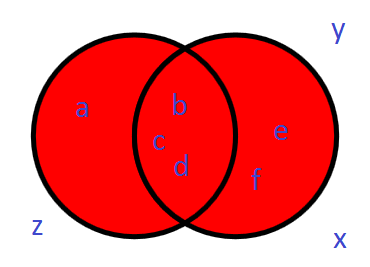
\includegraphics{sets-union.png}
\begin{figure}
\centering
\def\seta{(-1,0) circle (2)}
\def\setb{(1,0) circle (2)}
\begin{tikzpicture}
     \tikzstyle{element}=[minimum size=1mm, font=\large]
    \draw [fill=red]   \seta;
    \draw [fill=yellow]\setb;
    \begin{scope}[even odd rule]
        \clip \seta;
        \fill[fill=orange] \setb;
    \end{scope}
    \draw \seta;
    \draw \setb;
    \foreach \t/\x/\y in { z/-3/-2, x/3/-2, y/3/2, a/-2/0, b/-.1/1, c/.3/0, d/-.2/-1,
    e/2/.5, f/1.5/-.5 }
        \node[element] (\t) at (\x,\y) {$\t$};
\end{tikzpicture}
\caption{Пересечение двух множеств}
\end{figure}


Здесь $x$, $y$ и $z$ — это просто некоторые элементы, которые не вошли ни в одно из множеств. Всегда при работе со множествами (да и вообще всегда) важно рассматривать не только объекты, с которыми мы непосредственно работаем, но и внешние факторы. Красным цветом обозначено объединение двух множеств, представляемых кругами.

{\bfseries Определение.} Пересечением множеств $A$ и $B$ ($A\cap B$) называется множество, которое содержит лишь те элементы которые принадлежат сразу обоим множествам: $\forall x, (x\in A \wedge x \in B \leftrightarrow x\in A\cap B)$.

{\bfseries Пример.} Пусть $A = \{a, b, c, d\}$ и $B = \{b, c, d, e, f\}$. Тогда $A\cap B = \{b, c, d\}$

{\bfseries Упражнение.} Нарисуйте круги Эйлера для пересечения множеств (какую часть рисунка надо закрасить цветом?)

{\bfseries Определение.} Множества называются {\slshape непересекающимися}, если $A\cap B = \emptyset$ (то есть множества не имеют общих элементов). В противном случае множества называются пересекающимися.

{\bfseries Пример.} Множества $\{a, b, c\}$ и $\{d, e, f\}$ не пересекаются. Множества $\{a, b\}$ и $\{b, c\}$ пересекаются, и их пересечением является множество $\{b\}$.

{\bfseries Определение.} Разностью множеств $A\setminus B$ называется множество, содержащее все те элементы $A$, которые не содержатся в $B$: $\forall x, (x \in A\cap B \leftrightarrow x\in A \wedge x \not \in B)$.

{\bfseries Пример.} Пусть $A = \{a, b, c, d\}$ и $B = \{b, c, d, e, f\}$. Тогда $A\setminus B = \{a\}$

{\bfseries Упражнение.} Нарисуйте круги Эйлера для разности множеств.

{\bfseries Определение.} {\slshape Симметрической разностью} множеств $A\bigtriangleup B$ называется множество $(A\setminus B)\cup (B\setminus A)$, то есть множество элементов, принадлежащих либо $A$, либо $B$, но не их пересечению: $\forall x,(x\in A\bigtriangleup B \leftrightarrow x\in A \oplus x\in B)$.

{\bfseries Пример.} Пусть $A = \{a, b, c, d\}$ и $B = \{b, c, d, e, f\}$. Тогда $A\bigtriangleup B = \{a, e, f\}$.

{\bfseries Упражнение.} Нарисуйте круги Эйлера для симметрической разности множеств.

Часто при работе со множествами, мы держим в уме, что все элементы нашего множества являются элементами некоторого другого более крупного множества, содержащего все возможные объекты рассматриваемой нами задачи. Например, если мы говорим о множестве звёзд на небе, то мы можем держать в уме так же множество всех звезд вообще, а не только видимых нам. Если мы говорим о множестве учеников десятого класса школы N469, то как более общее множество мы можем подразумевать множество вообще всех учеников этой школы, либо же множество всех школьников страны, либо же множество всех людей. Смотря что за задачу мы решаем. Поэтому оказывается полезным ввести следующее определение:

{\bfseries Определение.} {\slshape Универсальным множеством}, или {\slshape универсумом}, называется множество всех возможных элементов, имеющих смысл в решаемой задаче.

{\bfseries Пример.} Если посмотреть на круги Эйлера, приведенные выше для иллюстрации объединения множеств и считать, что на картинке представлены все интересные нам элементы, то там универсумом в этом случае является множество $U = \{a, b, c, d, e, f, x, y, z\}$.

{\bfseries Определение.} {\slshape Дополнением} множества $A$ (обозначается как $A^C$) называется множество элементов универсума, не принадлежащих множеству $A$: $\forall x, x\in A^C \leftrightarrow x\in U \wedge x \not \in A$, где $U$ — универсум. Это же можно записать и без упоминания универсума, если предположить, что мы держим его «в уме»: $\forall x, x\in A^C \leftrightarrow x\not \in A$.

Понятно, что для операции дополнения необходимо строгое задание универсума, иначе она теряет смысл.

{\bfseries Пример.} Пусть $U = \{a, b, c, d, e, f, x, y, z\}$ и $A = \{a, b, c, d\}$. Тогда $A^C = \{e, f, x, y, z\}$.

{\bfseries Упражнение.} Нарисуйте круги Эйлера для дополнения.

Основные понятия мы определили, теперь надо разобраться с их свойствами. Однако прежде чем мы сформулируем нашу первую теорему о множествах, сделаем такое существенное наблюдение: практически все логические операции и операции над множествами находятся в соответствии друг с другом и операции над множествами определяются просто через логические операции. Так, логическое И задает пересечение множеств. Логическое ИЛИ — объединение. Исключающее ИЛИ — симметрическую разность. Отрицание высказываний — дополнение множеств. Эквиваленция — равенство множеств. Импликация — подмножества. В некотором смысле можно так же провести аналогию между универсумом и истинным высказыванием, а так же пустым множеством и ложным высказыванием.

Для продвинутых читателей, которые целиком осилили и поняли первую главу, отмечу, что сильно извратившись (как раз как я люблю), определить можно не только операции над множествами через операции над высказываниями, но и наоборот. Пусть, например, у нас есть теория $T_0$ и формулы $\phi$ и $\psi$. Пусть у нас так же есть теория $T_1$, для которой известно, что $\mathrm{Mod}(T_1) = \mathrm{Mod}(T_0, \phi) \cup \mathrm{Mod}(T_0, \psi)$. Тогда можно показать (сделайте это самостоятельно), что теория $T_1 = T_0 \cup \{\phi\vee \psi\}$ будет иметь как раз требуемое множество моделей (хотя такая теория может быть конечно не единственна), и именно через свойства моделей при добавлении формул можно определить логическое ИЛИ. Нечто аналогичное мы делали, когда определяли понятие импликации. Нечто аналогичное можно сделать и для всех других логических операций.

{\bfseries Теорема 1}. Для операций над множествами справедливы следующие законы:

{\slshape Ассоциативность:}

1) $(A \cap B) \cap C = A \cap (B \cap C)$

2) $(A \cup B) \cup C = A \cup (B \cup C)$

3) $(A \bigtriangleup B) \bigtriangleup C = A \bigtriangleup (B \bigtriangleup C)$

{\slshape Коммутативность:}

4) $A \cap B = B \cap A$

5) $A \cup B = B \cup A$

6) $A \bigtriangleup B = B \bigtriangleup A$

7) $A = B$ равносильно $B = A$.

{\slshape Дистрибутивность:}

8) $A \cap (B \cup C) = (A \cap B) \cup (A \cap C)$

9) $A \cup (B \cap C) = (A \cup B) \cap (A \cup C)$

10) $A \cap (B \bigtriangleup C) = (A \cap B) \bigtriangleup (A \cap C)$

{\slshape Двойное дополнение:}

11) $(A^C)^C = A$

{\slshape Законы де Моргана:}

12) $(A \cap B)^C = A^C \cup B^C$

13) $(A \cup B)^C =A^C \cap B^C$

{\slshape Еще по мелочам (здесь $U$ — универсальное множество):}

14) $A \cap U = A$

15) $A \cap \emptyset = \emptyset$

16) $A \cup U = U$

17) $A \cup \emptyset = A$

18) $A \bigtriangleup \emptyset = A$

19) $A \bigtriangleup U = A^C$

20) $A \cap A^C = \emptyset$

21) $A \cup A^C = U$

22) $A \bigtriangleup A^C = U$

23) $A\cap A = A$

24) $A\cup A = A$

25) $A \bigtriangleup A = \emptyset$

26) $A \cap (A^C \cup B) = A \cap B$

27) $A \cup (A^C \cap B) = A \cup B$

{\slshape Новенькое для отрицания:}

28) $A \setminus B = A \cap B^C$

{\slshape Свойства подмножеств:}

29) Если $A \not \subset B$, то $A$ и $B^C$ пересекаются.

30) $A \subset A$

31) Транзитивность: $A \subset B \wedge B \subset C \rightarrow A \subset C$ (думаю на всякий случай это свойство полезно проговорить словами: если $A\subset B$ и $B\subset C$, то $A\subset C$)

32) $A \subset B\cap C \rightarrow A \subset B$

33) Если $A \subset B$, то $B^C \subset A^C$ и наоборот.

{\bfseries Доказательство.} Во-первых, как можно заметить, все эти свойства дублируют соответствующие свойства для логических операций. Такой вот поворот событий. Некоторые свойства пришлось немного переформулировать (в основном в части с импликацией), одно свойство добавилось для разности множеств, несколько свойств потеряли смысл в теории множеств либо стали неинтересны. Но в целом мы имеем то же самое один в один.

Доказательства всех этих свойств оказываются совершенно элементарны и сводятся, как можно догадаться, к простой переформулировке на языке логики. Давайте докажем, например свойство 10 (мы здесь активно используем задание подмножеств предикатами, которые в нашем случае являются простой логической формулой, а так же дистрибутивность из теоремы 1 главы 1):

$A \cap (B \bigtriangleup C) = \{x|x\in A \wedge x \in B\bigtriangleup C\} = \{x|x\in A \wedge (x \in B \oplus x \in C)\}\\ = \{x|(x\in A \wedge x \in B) \oplus (x \in A \wedge x \in C)\} = \{x|(x\in A \cap B) \oplus (x \in A \cap C)\} \\ = \{x|x\in (A \cap B) \bigtriangleup (A \cap C)\} = (A \cap B) \bigtriangleup (A \cap C)$

Что и требовалось. Как видно из этих рассуждений, операции над множествами и операции над высказываниями — это действительно очень близкие понятия, которые во многом отражают одно и то же, только несколько под разным углом.

Остальные свойства докажите самостоятельно в качестве упражнения, а так же нарисуйте круги Эйлера для этих свойств — они должны дать довольно не плохую интуицию относительно свойств множеств (и заодно логики). \qed

В завершение параграфа определим еще одну операцию, которая уже не имеет никакого прообраза в логике.

{\bfseries Определение.} {\slshape Булеаном} множества $A$ (обозначается $2^A$) называется множество всех его подмножеств.

{\bfseries Пример.} Пусть $A = \{a, b, c\}$. Тогда $2^A = \{\emptyset, \{a\}, \{b\}, \{c\}, \{a, b\}, \{a, c\}, \{b, c\}, A\}$.

Обратите внимание, что всегда $\emptyset \in 2^A$ и $A\in 2^A$. Так же обратите внимание на то, что булеан, сам являясь множеством, содержит в качестве своих элементов другие множества (это ничему не противоречит — элементами множеств могут быть и другие множества, почему бы и нет?).

Так же важно отметить такой нюанс: если $a \in A$, то $\{a\} \in 2^A$, но $a \not \in 2^A$. Это довольно очевидно: $a\not = \{a\}$, ведь множество состоящее из одного элемента и сам этот элемент логически разные сущности.

Понятие булеана будет активно использоваться нами в дальнейшем, а пока мы рассмотрим опять же аналогию булеана с логикой (это только для дотошных читателей). Пусть $A$ — некоторое одноэлементное множество. Тогда $2^A = \{\emptyset, A\}$.Теперь, если рассматривать наши операции над множествами, ограничившись лишь этим булеаном, то если назвать $\emptyset$ ложью, а $A$ истиной, то наша аналогия между логическими операциями и операциями над множествами станет уже не примерной, а совершенно однозначной.

Таким образом можно считать, что логика — это в некотором смысле частный случай теории множеств, которая в свою очередь является обобщением логики. Если рассматривать $A$, который состоит из многих элементов, то можно в некотором смысле говорить, что $2^A$ — это модель нечеткой логики, где $A$ — истинное высказывание, $\emptyset$ — ложное высказывание, а остальные множества являются истинными высказываниями лишь с некоторой степенью вероятности. Это далеко не самый удобный подход для определения нечеткой логики, и на практике математиками не используется наверное никогда, кроме очень узких областей, однако мы будем иногда обращаться к этому примеру в качестве иллюстраций и более интуитивного понимания отдельных понятий.

Так же у дотошного читателя может возникнуть определенный дискомфорт от той последовательности изложения, которую он до сих пор наблюдает: говоря о логике и предикатах мы ввели понятие множеств, говоря о множествах мы во всю опирались на логигу. Это как в России: чтобы получить работу по специальности, надо иметь опыт работы по этой специальности, а чтобы получить опыт, надо проработать по этой специальности. Такие ситуации допустимы в быту, но не в науке, поэтому порочные круги необходимо разрывать.

Пока я стараюсь дать просто интуицию о множествах, поскольку строгое формальное изложение без порочных кругов и без начальной интуиции вряд ли окажется сильно полезно и понятно читателю. Поэтому пока мы оставим все как есть, а формальное изложение проведем в конце главы, где уже окончательно расставим все на свои места и избавимся от всех неточностей и нечеткости в определениях.

\section{Отношения}

{\bfseries Определение.} {\slshape Упорядоченным набором}, или же {\slshape кортежем}, или же {\slshape отношением}, называется набор объектов, в котором так же определен порядок этих объектов.

Как обычно это совершенно чудовищное определение, которое не может считаться строгим математическим, но пока мы попробуем работать с ним, напирая на интуицию, а не научную строгость. Записывается упорядоченный набор как $(a, b, \ldots, z)$, где элементы $a$, $b$ и $z$ являются элементами некоторых определенных множеств.

Как более-менее практический пример можно рассмотреть базы данных. Чтобы не говорить слишком абстрактно, а рассмотреть более конкретную ситуацию, можно рассмотреть простую записную книжку мобильного телефона, которая тоже по сути является компьютерной базой данных.

Сама база данных представляет из себя множество записей, каждая из которых состоит из нескольких полей. Это можно представить как таблицу:

\begin{table}[h]
\begin{tabular}{lllll}
Фамилия & Имя & Телефон & ДР & Комментарий\\
Авраам & Линкольн & +1(270)... & 12.02.1802 & Президент\\
Бенито & Муссолини & +3(39)... & 29.07.1883 & Фашик\\
Владимир & Ленин & +7(499)... & 22.04.1870 & Свой мужик\\
Григорий & Распутин & +7(3459)... & 21.01.1869 & Есть чему завидовать\\
Джорджина & Байер & +6(64)... & 11.1957 & Транссексуал\\
... & ... & ... & ... & ...
\end{tabular}
\end{table}

Если предположить, что $F$ — множество фамилий, $N$ — множество имен, $P$ — множество телефонов, $D$ — множество дат календаря и $S$ — множество произвольных текстовых строк, то можно сказать, что данная таблица иллюстрирует множество упорядоченных наборов следующего вида:

$\{(f, n, p, b, c)|f\in F, n \in N, p \in P, b \in D, c \in S\}$

(Строго говоря с точки зрения логики правильнее было бы писать не символ запятой справа в предикате, а символ $\wedge$, но чаще в случаях, подобных нашему, употребляется именно запятая в силу большей наглядности и удобства — означает она при этом логическое И).

Практически вся теория баз данных построена на самом деле на теории множеств в рамках того, что я уже рассказал, и декартова произведения, о котором речь пойдет ниже. База данных — это множество, элементами которого являются упорядоченные наборы. Команды работы с базой данных — это операции, задающие предикаты и операции над множествами. Я не могу позволить себе углубляться сейчас в алгебру реляционных баз данных и синтаксис языка SQL, но вообще рекомендую всем читателям с этими вещами ознакомиться — будет небесполезно, а заодно увидите кучу примеров тому, о чем я сейчас говорю.

Здесь стоит еще сделать такое наблюдение по терминологии. Чаще всего термин кортеж применяется именно в теории баз данных, термин отношение применяется чаще всего в случае упорядоченных пар, в которых оба элемента принадлежат одному и тому же множеству $\{(x, y)|x\in A, y\in A\}$, а термин упорядоченный набор используется в остальных случаях. Здесь нет строгого формального разграничения, это просто сложившаяся практика, которая однако может часто нарушаться и в этом нет ничего преступного.

{\bfseries Определение.} {\slshape Декартовым}, или {\slshape прямым}, {\slshape произведением} множеств $A$ и $B$ называется множество $A\times B = \{(a, b)|a\in A, b\in B\}$.

Говоря человеческим языком, $A\times B$ — это множество всех возможных упорядоченных пар $(a, b)$, таких что $a\in A$ и $b \in B$.

{\bfseries Пример.} Пусть $A = \{0, 1\}$, а $B = \{a, b, c\}$. Тогда $A\times B = \{(0, a), (0, b), (0, c), (1, a), (1, b), (1, c)\}$.

Кое-какую интуицию относительно декартова произведения вероятно поможет развить иллюстрация в виде таблицы. Столбцы в ней отводятся для элементов одного множества, строки — для другого множества, а на пересечении стоит их декартово произведение:

$\begin{array}{c|ccc}\times & a&b&c\\ \hline 0 & (0,a) & (0, b) & (0, c) \\ 1 & (1, a)& (1, b) &(1, c)\end{array}$

{\bfseries Пример.} Часто с помощью декартова произведения можно описывать какие-то физические понятия. Пусть $A$ — множество мастей (червы, буби, крести, трефы), а $B$ — множество достоинств (6, 7, 8, ..., король, туз). Тогда $A \times B$ — множество игральных карт в колоде.

{\bfseries Упражнение.} Покажите, что в общем случае $A\times B \not = B \times A$. В каких частных случаях все же $A\times B = B \times A$?

Легко заметить, что $(A\times B)\times C \not= A\times (B \times C)$, поскольку в случае множества до знака равенства будут получаться пары вида $((a, b), c)$, а для множества справа от знака равенства будут пары $(a, (b, c))$. Однако как и раньше удобно считать, что произведение $A\times B\times C$ без скобок дает нам упорядоченные тройки $(a, b, c)$ так же без каких-либо специальных группировок. Для удобства часто, впрочем, считают, что и при наличии скобок декартово произведение дает обычные упорядоченные наборы: $(A\times B)\times C = \{(a, b, c)|a\in A, b\in B, c\in C\}$.

Каждое отношение таким образом является подмножеством декартова произведения $\rho \subset X\times X$ — в этом параграфе нас будут интересовать как раз такие отношения. Часто для удобства применяется так же следующая запись: если $(x, y) \in \rho$, то пишут $x\rho y$. Из последующего текста будет видно почему это удобно.

{\bfseries Пример.} Пусть $S$ — множество высказываний. Тогда любая логическая операция задает отношение на этом множестве. В простейшем случае, если рассматривать только одно истинное и ложное высказывание $S = \{0, 1\}$, то $\vee = \{(1, 0), (0, 1), (1, 1)\}$, $\leftrightarrow = \{(0, 0), (1, 1)\}$ и так далее. По аналогии любому предикату на множествах можно сопоставить в соответствие некоторое отношение (возможно, не из двух элементов).

{\bfseries Определение.} Отношение называется {\slshape рефлексивным}, если для любого $x$ выполняется $x\rho x$.

{\bfseries Определение.} Отношение называется {\slshape антирефлексивным}, если для любого $x$ отношение $x\rho x$ не имеет места быть.

{\bfseries Определение.} Отношение называется {\slshape транзитивным}, если для любых $x$, $y$ и $z$ из того, что $x\rho y$ и $y \rho z$ следует, что $x\rho z$.

{\bfseries Определение.} Отношение называется {\slshape симметричным}, если из того, что $x\rho y$ следует $y\rho x$.

{\bfseries Определение.} Отношение называется {\slshape антисимметричным}, если из того, что $x \rho y$ и $y \rho x$ следует, что $x = y$.

Можно привести и больше возможных общих свойств отношений, но для наших нужд достаточно и того что я уже привел.

{\bfseries Упражнение.} Запишите эти свойства на языке логики.

{\bfseries Упражнение}. Приведите пример нетранзитивного отношения на множестве $\{0, 1\}$.

{\bfseries Определение.} Отношение называется {\slshape отношением эквивалентности}, если оно рефлексивно, транзитивно и симметрично.

Отношение эквивалентности часто обозначается символами $=$, $\approx$, $\sim$ и подобными (хотя есть и другие обозначения, которые мы будем по ситуации использовать). Если на множестве задано несколько отношений эквивалентности, то символьное обозначение отношения часто указывается справа внизу от знака эквивалентности: $\approx_R$.

{\bfseries Упражнение.} Пусть $S$ — множество учеников средней школы №469. Отношение $x\approx_Y y$ означает, что ученики $x$ и $y$ заканчивают школу в одном году, отношение $x \approx_C y$ означает, что они учатся в одном классе, $x \sim y$ что имеют одинаковую успеваемость. Проверьте, что все заданные отношения — это отношения эквивалентности (для этого необходимо проверить, что они рефлексивны, транзитивны и симметричны).

Следующие три упражнения уже посложнее, и их начинающие могут пропустить.

{\bfseries Упражнение.} Пусть $S$ — некоторое множество, а $P$ — множество предикатов, определенных на этом множестве. Пусть нам задано такое отношение, что $p \approx q$ тогда и только тогда, когда $p$ и $q$ определяют одинаковые подмножества $S$. Докажите, что это отношение эквивалентности.

{\bfseries Упражнение.} Пусть нам задано множество логических формул, все с одинаковым числом параметров. Отношение $f=g$ определено для функций, которые на одинаковых значениях параметров принимают одинаковые значения истинности. Докажите, что это отношение эквивалентности.

{\bfseries Упражнение.} Пусть нам задана некоторая теория. Докажите, что семантическая эквивалентность формул является отношением эквивалентности. (Напомню, что формулы $\phi$ и $\psi$ семантически эквивалентны, если в любой модели теории $\psi\leftrightarrow\phi$).

Примеры, приведенные в упражнении, демонстрируют основную идею отношения эквивалентности: это набор пар, которые имеют какие-то общие характеристики, которые и отражают отношение. Причем мыслить об отношении как о парах элементов чаще всего не удобно с интуитивной точки зрения — удобнее мыслить об отношении эквивалентности именно как о наличии какого-то общего свойства.

{\bfseries Определение.} Пусть дано множество $A$ и на нем задано отношение эквивалентности $\sim$. Множество всех элементов $x$, для которых $a\sim x$ называется {\slshape классом эквивалентности} элемента $a$ и обозначается как $[a]$.

{\bfseries Теорема.} Для любых элементов $a, b \in A$ классы эквивалентности $[a]$ и $[b]$ либо совпадают, либо не пересекаются.

{\bfseries Доказательство.} Проведем доказательство от противного и предположим, что теорема неверна. Пусть классы эквивалентности $[a]$ и $[b]$ пересекаются, но не совпадают. Тогда найдется элемент $x$, принадлежащий сразу обоим классам эквивалентности, и элемент $b' \in [b]$, такой что $b' \not\in [a]$. Для него однако верно, что $b' \sim x$, но поскольку $x \in [a]$ и $x\sim a$, то в силу транзитивности $b' \sim a$ и соответственно $b' \in [a]$. Полученное противоречие говорит, что наше предположение «от противного» было не верно, и значит теорема верна. \qed

Это доказательство на первый взгляд может показаться странным и непонятным — вспомните тогда свойства импликации $(a\rightarrow b) \leftrightarrow (\neg b \rightarrow \neg a)$ и как она связана с выводимостью (см. §1.6).

Смыслом теоремы является тот факт, что каждое множество с заданным на нем отношением эквивалентности можно разбить на непересекающиеся классы эквивалентности.

{\bfseries Пример.} Пусть опять $S$ — множество учеников школы №469. Всех учеников можно сгруппировать по классам, по успеваемости или по году окончания школы. Пусть $A$ — множество двоечников, $B$ — троечников, $C$ — хорошистов и $D$ — отличников. Очевидно, что эти множества не пересекаются и $S = A\cup B\cup C\cup D$, причем любые два ученика из одного и того же множества находятся в отношении $\sim$ («имеют одинаковую успеваемость») друг с другом, а ученики из разных множеств в этом отношении не находятся.

{\bfseries Определение.} Процесс разбиения множества на классы эквивалентности называется {\slshape факторизацией}, а само множество классов эквивалентности называется {\slshape фактор-множеством}. Если $\rho$ — отношение эквивалетности на $A$, то фактормножество $A$ по $\rho$ обозначается как $A/\rho$.

{\bfseries Пример.} Продолжая пример с успеваемостью, можно записать, что $S/\sim = \{A, B, C, D\}$.

Обратите внимание в какую сторону рисуется черта фактормножества и не путайте ее с разностью множеств. $A\setminus B$ — разность, а $A/\rho$ — факторизация.

Интуитивно таким образом можно рассматривать факторизацию как разбиение множества на подмножества в соответствии с некоторым отношением («фактором»). Обратное кстати тоже верно — если множество разбито на непересекающиеся подмножества, то по ним можно задать отношение эквивалентности.

{\bfseries Упражнение.} Пусть $A = \{a, b, c, d\}$ разбито на подмножества $\{a, b\}$ и $\{c, d\}$. Запишите по этому разбиению отношение эквивалентности $\rho$ как множество упорядоченных пар (начинается эта запись как $\rho = \{(a, a), (a, b), \ldots\}$).

Перейдем теперь ко второму не менее важному отношению, которое мы сравнительно часто будем использовать.

{\bfseries Определение.} Отношение называется {\slshape отношением частичного порядка} (или {\slshape отношением нестрогого частичного порядка}), если оно рефлексивно, транзитивно и антисимметрично.

{\bfseries Определение.} Отношение называется {\slshape отношением строгого частичного порядка}, если оно антирефлексивно, транзитивно и антисимметрично.

Отношение частичного порядка удобно обозначать как $\le$. Отношение строго частичного порядка как $<$. Если $a \le b$ и $a \not= b$, то $a<b$. Если $b \le a$, то можно писать $a \ge b$ или $a > b$, если $a\not= b$. Легко видеть, что отношения частичного и строгого частичного порядка — это фактически одного и то же. Различаются они лишь тем, находится ли каждый элемент в отношении с самим собой (то есть можем ли мы записать отношение $x\le x$). В теории в основном используется отношение частичного порядка, в конкретных задачах часто может оказаться удобным и то и другое. Хотя погоды это разграничение не делает: если у нас есть строгий порядок, то его всегда можно сделать не строгим, дополнив парами $x\le x$, и наоборот нестрогий порядок можно сделать строгим, выкинув такие пары.

{\bfseries Упражнение.} Докажите, что если элементами множества являются множества (например, это булеан), то отношение $\subset$ является отношением частичного порядка.

{\bfseries Упражнение.} Докажите, что отношение «является предком» на множестве людей является строгим частичным порядком.

{\bfseries  Упражнение.} Докажите, что отношение «не ниже чем» на множестве всех людей образует нестрогий частичный порядок, а отношение «выше чем» строгий частичный порядок.

{\bfseries Упражнение.} Покажите, что отношение «является родителем» не является отношением частичного порядка.

{\bfseries Упражнение.} Покажите, что на множестве картонных коробок отношение «влезает в» является отношением строгого частичного порядка.

{\bfseries Упражнение.} Рассмотрим множество всех логических функций с одинаковым числом параметров. Определим на них отношение следующим образом: $f\le g$ тогда и только тогда, когда на одинаковых наборах параметров либо эти функции принимают одинаковое значение, либо $f=0$, а $g=1$. Докажите, что отношение частичного порядка. Как оно соотносится с порядком на булеане множества?

{\bfseries Пример.} В микроэкономике рассматриваются отношения предпочтений, задаваемые на множествах альтернатив (читай товаров). Считается, что потребители могут сравнивать альтернативы по степени предпочтительности и данное отношение является как раз отношением частичного порядка. (Психологи однако доказывают, что предпочтения людей не являются рациональными и таким образом не образуют частичный порядок на множестве товаров).

Отношение частичного порядка удобно представлять в виде диаграмм. Например, так будет выглядеть диаграмма для булеана множества $\{x, y, z\}$:

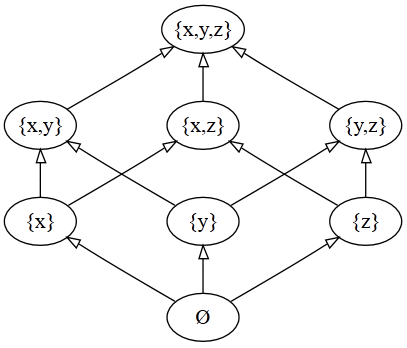
\includegraphics{hasse1.png}

(Картинка из Википедии, свободной энциклопедии, потому что сам не умею пока такие рисовать; LibreOffice Draw не справляется с задачей).

Здесь стрелка обозначает отношение «является подмножеством». Элементы, располагающиеся выше, оказываются «больше» элементов, располагающихся внизу, если между ними есть путь из стрелок. Если на диаграмме есть стрелка $a\to b$ и стрелка $b\to c$, то по транзитивности должна быть и стрелка $a\to c$, которая не указывается, чтобы не загромождать картинку.

Отношение частичного порядка таким образом упорядочивает элементы множества. Существенно, однако, что если задан частичный порядок, то совершенно не факт, что удастся сравнить произвольные два объекта. Как видно из диаграммы выше, элементы $\{x, y\}$ и $\{z\}$ не сравнимы между собой. Точно так же для любых двух людей не обязательно кто-то один из них должен быть предком другого, и в этом смысле не сравнимыми являются брат и сестра.

{\bfseries Определение.} {\slshape Линейным порядком} называется отношение частичного порядка, относительно которого сравнимы любые два элемента множества.

{\bfseries Пример.} Отношение «не ниже чем» является линейным порядком на множестве людей.

{\bfseries Определение.} {\slshape Максимальным элементом} называется такой элемент, что не существует элемента, большего него.

{\bfseries Определение.} {\slshape Наибольшим элементом} называется такой элемент, что он больше любого другого элемента.

{\bfseries Пример.} На множестве коробок максимальным элементом будет коробка, которая не может влезть ни в какую другую коробку. Наибольшим элементом будет коробка, в которую может поместиться любая другая коробка.

В полной аналогии можно ввести понятия {\slshape минимального} и {\slshape наименьшего элемента}, но мы не будем на это отвлекаться, так там вся теория совершенно аналогична.

Очевидно, что если множество обладает наибольшим элементом, то он же будет и единственным максимальным элементом. Однако же максимальных элементов может быть несколько, и наибольшего элемента в этом случае не будет, как в случае следующей диаграммы:

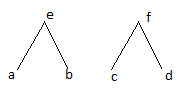
\includegraphics{maxelement.png}

(На этот раз рисовал сам; извиняюсь за качество — я математик, а не художник; я когда-нибудь научусь и переделаю это убожество).

На приведенной диаграмме два максимальных элемента: $e$ и $f$. Наибольшего элемента нет. На следующей же диаграмме уже имеется один наибольший элемент $g$, он же является и максимальным:

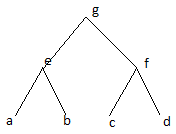
\includegraphics{hielement.png}

(Я правда надеюсь, что мне кто-нибудь из читателей поможет с иллюстрациями).

В обоих этих примерах порядки не являлись линейными. В случае же линейного порядка, очевидно, что понятия максимального и наибольшего элемента совпадают.

{\bfseries Определение.} {\slshape Верхней гранью} подмножества $S\subset U$ называется такой элемент $x\in U$, что для любого элемента $s\in S$ выполняется $s \le x$.

{\bfseries Определение.} {\slshape Нижней гранью} подмножества $S\subset U$ называется такой элемент $x\in U$, что для любого элемента $s\in S$ выполняется $s \ge x$.

Если $x$ — верхняя грань подмножества $S$, то любой элемент больший $x$ так же будет являться верхней гранью $S$. Таким образом, верхние грани сами по себе образуют множество (аналогично с нижними) и есть смысл ввести следующие определения:

{\bfseries Определение.} {\slshape Наименьшей}, или {\slshape точной}, {\slshape верхней гранью}, называется наименьшая из верхних граней. Обозначается она как $\sup S$.

{\bfseries Определение.} {\slshape Наибольшей}, или {\slshape точной}, {\slshape нижней гранью}, называется наибольшая из нижних граней. Обозначается она как $\inf S$.

(С этого места начинаются абстракции, которые начинающему читателю вероятно и не являются необходимыми — если будет не понятно о чем речь, можно смело пропускать. Если однако разобраться с материалом, то это будет хорошим упражнением для ума.)

Если подмножество $S$ состоит лишь из двух элементов, то операции «точных граней» можно рассматривать как арифметические операции над этими элементами. В этом случае используется запись $\sup\{a, b\} = a\vee b$ и $\inf\{a, b\} = a\wedge b$.

{\bfseries Упражнение.} Докажите, что на булеане относительно порядка, образованного включением множеств, $A\wedge B = A\cap B$ и $A\vee B = A \cup B$ и они обладают соответственно всеми свойствами логического И и логического ИЛИ.

Сформулированное в упражнении утверждение в общем случае неверно, если рассматривать произвольный частичный порядок. Во-первых, могут не выполняться сами свойства логических операций, а во-вторых самих точных граней может и не быть. Поэтому вводятся следующие определения:

{\bfseries Определение.} {\slshape Решёткой} называется частично упорядоченное множество, у которого для любого двухэлементного подмножества существуют точные верхние и нижние грани.

{\bfseries Определение.} {\slshape Дистрибутивной решёткой} называется решётка, для которой оказываются верны свойства дистрибутивности операций $\wedge$ и $\vee$ (см §1.1, теорема 1).

{\bfseries Упражнение.} Докажите, что решётка, изображенная на диаграмме ниже, не является дистрибутивной:

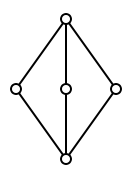
\includegraphics{lattice.png}

Дистрибутивные решетки уже практически дублируют законы логики, которым была посвящена первая глава. Не достает только $1$ и $0$. Следующие определения исправляют ситуацию:

{\bfseries Определение.} Решетка называется ограниченной, если в ней существуют наибольший и наименьший элементы, обозначаемые соответственно как $0$ и $1$.

{\bfseries Упражнение.} Если решетка имеет минимальный или максимальный элементы, то они будут единственны и будут являться наименьшим и наибольшим элементами. Докажите это.

{\bfseries Определение.} {\slshape Дополнением} элемента $x$ ограниченной решетки такой элемент $y$, что $x\wedge y = 0$ и $x \vee y = 1$. Дополение $x$ обозначается как $\neg x$.

{\bfseries Определение.} Если в решетке каждый элемент обладает дополнением, то такая решетка называется {\slshape решеткой с дополнением}.

{\bfseries Определение.} {\slshape Булевой алгеброй} называется дистрибутивная решетка, обладающая наименьшим и наибольшим элементами (обозначаемыми соответственно $0$ и $1$).

{\bfseries Пример.} Если рассмотреть двухэлементное множество $\{0, 1\}$ и определить на нем порядок $0 < 1$, то мы получим в точности классическую логику, которую рассматривали в первой главе, которая как теперь видно является разновидностью булевой алгебры.

{\bfseries Пример.} Булеан любого множества $A$ задает булеву алгебру относительно включения множеств, где наибольшим элементом является само множество $A$, а наименьшим пустое множество.

{\bfseries Упражнение.} Для булевых алгебр справедливы все законы логики, которые мы приводили в теореме 1.1. Докажите это.

Если у нас есть два частично упорядоченных множества $A$ и $B$, то на их декартовом произведении можно задать частичный порядок несколькими способами:

{\bfseries Определение.} {\slshape Лексигографическим порядком} на $A\times B$ называется порядок, при котором $(a, b) \le (a', b')$ либо когда $a < a'$, либо когда $a=a'$ и $b\le b'$.

{\bfseries Определение.} {\slshape Естественным порядком} на $A\times B$ называется порядок, при котором $(a, b) \le (a', b')$ тогда и только тогда, когда одновременно $a \le a'$ и $b \le b'$.

Оба этих порядка естественно распространяются на декартово произведение любого количества множеств.

{\bfseries Упражнение.} Пусть $B = \{0, 1\}$ и на нем введен порядок $0 < 1$. Будем рассматривать множество $B\times B\times \ldots \times B$ (фактически упорядоченные наборы единиц и нулей) с естественным частичным порядком. Докажите, что такой частичный порядок задает булеву алгебру (кстати, как раз ту самую, которая повсеместно используется в программировании и называется там побитовыми логическими операциями).

{\bfseries Упражнение.} Докажите, что линейно-упорядоченное множество является дистрибутивной решеткой, и соответственно при наличии наименьшего и наибольшего элемента является булевой алгеброй.

{\bfseries Упражнение.} Является ли булевой алгеброй множество $B\times B \times \ldots \times B$, введенное выше, относительно лексикографического порядка?

{\bfseries Упражнение.} Пусть теперь $B$ — некоторая произвольная булева алгебра. Является ли булевой алгеброй $B\times B \times \ldots \times B$ относительно лексикографического порядка? А относительно естественного порядка?



\end{document}
